% ******************************* PhD Thesis Template **************************
% Please have a look at the README.md file for info on how to use the template

\documentclass[a4paper,12pt,times,numbered,print,index,custommargin]{Classes/PhDThesisPSnPDF}

% ******************************************************************************
% ******************************* Class Options ********************************
% *********************** See README for more details **************************
% ******************************************************************************

% `a4paper'(The University of Cambridge PhD thesis guidelines recommends a page
% size a4 - default option) or `a5paper': A5 Paper size is also allowed as per
% the Cambridge University Engineering Deparment guidelines for PhD thesis
%
% `11pt' or `12pt'(default): Font Size 10pt is NOT recommended by the University
% guidelines
%
% `oneside' or `twoside'(default): Printing double side (twoside) or single
% side.
%
% `print': Use `print' for print version with appropriate margins and page
% layout. Leaving the options field blank will activate Online version.
%
% `index': For index at the end of the thesis
%
% `draftclassic': For draft mode without loading any images (same as draft in book)
%
% `draft': Special draft mode with line numbers, images, and water mark with
% timestamp and custom text. Position of the text can also be modified.
%
% `abstract': To generate only the title page and abstract page with
% dissertation title and name, to submit to the Student Registry
%
% `chapter`: This option enables only the specified chapter and it's references
%  Useful for review and corrections.
%
% ************************* Custom Page Margins ********************************
%
% `custommargin`: Use `custommargin' in options to activate custom page margins,
% which can be defined in the preamble.tex. Custom margin will override
% print/online margin setup.
%
% *********************** Choosing the Fonts in Class Options ******************
%
% `times' : Times font with math support. (The Cambridge University guidelines
% recommend using times)
%
% `fourier': Utopia Font with Fourier Math font (Font has to be installed)
%            It's a free font.
%
% `customfont': Use `customfont' option in the document class and load the
% package in the preamble.tex
%
% default or leave empty: `Latin Modern' font will be loaded.
%
% ********************** Choosing the Bibliography style ***********************
%
% `authoryear': For author-year citation eg., Krishna (2013)
%
% `numbered': (Default Option) For numbered and sorted citation e.g., [1,5,2]
%
% `custombib': Define your own bibliography style in the `preamble.tex' file.
%              `\RequirePackage[square, sort, numbers, authoryear]{natbib}'.
%              This can be also used to load biblatex instead of natbib
%              (See Preamble)
%
% **************************** Choosing the Page Style *************************
%
% `default (leave empty)': For Page Numbers in Header (Left Even, Right Odd) and
% Chapter Name in Header (Right Even) and Section Name (Left Odd). Blank Footer.
%
% `PageStyleI': Chapter Name next & Page Number on Even Side (Left Even).
% Section Name & Page Number in Header on Odd Side (Right Odd). Footer is empty.
%
% `PageStyleII': Chapter Name on Even Side (Left Even) in Header. Section Number
% and Section Name in Header on Odd Side (Right Odd). Page numbering in footer

% Uncomment to change page style
%\pagestyle{PageStyleII}

% ********************************** Preamble **********************************
% Preamble: Contains packages and user-defined commands and settings
% ******************************************************************************
% ****************************** Custom Margin *********************************

% Add `custommargin' in the document class options to use this section
% Set {innerside margin / outerside margin / topmargin / bottom margin}  and
% other page dimensions
\ifsetCustomMargin
  \RequirePackage[left=37mm,right=30mm,top=35mm,bottom=30mm]{geometry}
  \setFancyHdr % To apply fancy header after geometry package is loaded
\fi

% Add spaces between paragraphs
\setlength{\parskip}{0.2em}
% Ragged bottom avoids extra whitespaces between paragraphs
\raggedbottom
% To remove the excess top spacing for enumeration, list and description
%\usepackage{enumitem}
%\setlist[enumerate,itemize,description]{topsep=0em}

% *****************************************************************************
% ******************* Fonts (like different typewriter fonts etc.)*************

% Add `customfont' in the document class option to use this section

\ifsetCustomFont
  % Set your custom font here and use `customfont' in options. Leave empty to
  % load computer modern font (default LaTeX font).
  %\RequirePackage{helvet}

  % For use with XeLaTeX
  %  \setmainfont[
  %    Path              = ./libertine/opentype/,
  %    Extension         = .otf,
  %    UprightFont = LinLibertine_R,
  %    BoldFont = LinLibertine_RZ, % Linux Libertine O Regular Semibold
  %    ItalicFont = LinLibertine_RI,
  %    BoldItalicFont = LinLibertine_RZI, % Linux Libertine O Regular Semibold Italic
  %  ]
  %  {libertine}
  %  % load font from system font
  %  \newfontfamily\libertinesystemfont{Linux Libertine O}
\fi

% *****************************************************************************
% **************************** Custom Packages ********************************

% ************************* Algorithms and Pseudocode **************************

%\usepackage{algpseudocode}


% ********************Captions and Hyperreferencing / URL **********************

% Captions: This makes captions of figures use a boldfaced small font.
%\RequirePackage[small,bf]{caption}

\RequirePackage[labelsep=space,tableposition=top]{caption}
\renewcommand{\figurename}{Fig.} %to support older versions of captions.sty


% *************************** Graphics and figures *****************************

%\usepackage{rotating}
%\usepackage{wrapfig}

% Uncomment the following two lines to force Latex to place the figure.
% Use [H] when including graphics. Note 'H' instead of 'h'
%\usepackage{float}
%\restylefloat{figure}

% Subcaption package is also available in the sty folder you can use that by
% uncommenting the following line
% This is for people stuck with older versions of texlive
%\usepackage{sty/caption/subcaption}
\usepackage{subcaption}

% ********************************** Tables ************************************
\usepackage{booktabs} % For professional looking tables
\usepackage{multirow}

%\usepackage{multicol}
%\usepackage{longtable}
%\usepackage{tabularx}


% *********************************** SI Units *********************************
\usepackage{siunitx} % use this package module for SI units


% ******************************* Line Spacing *********************************

% Choose linespacing as appropriate. Default is one-half line spacing as per the
% University guidelines

% \doublespacing
% \onehalfspacing
% \singlespacing


% ************************ Formatting / Footnote *******************************

% Don't break enumeration (etc.) across pages in an ugly manner (default 10000)
%\clubpenalty=500
%\widowpenalty=500

%\usepackage[perpage]{footmisc} %Range of footnote options


% *****************************************************************************
% *************************** Bibliography  and References ********************

\usepackage{cleveref} %Referencing without need to explicitly state fig /table

% Add `custombib' in the document class option to use this section
\ifuseCustomBib
   \RequirePackage[square, sort, numbers, authoryear]{natbib} % CustomBib

% If you would like to use biblatex for your reference management, as opposed to the default `natbibpackage` pass the option `custombib` in the document class. Comment out the previous line to make sure you don't load the natbib package. Uncomment the following lines and specify the location of references.bib file

%\RequirePackage[backend=biber, style=numeric-comp, citestyle=numeric, sorting=nty, natbib=true]{biblatex}
%\addbibresource{References/references} %Location of references.bib only for biblatex, Do not omit the .bib extension from the filename.

\fi

% changes the default name `Bibliography` -> `References'
\renewcommand{\bibname}{References}


% ******************************************************************************
% ************************* User Defined Commands ******************************
% ******************************************************************************

% *********** To change the name of Table of Contents / LOF and LOT ************

%\renewcommand{\contentsname}{My Table of Contents}
%\renewcommand{\listfigurename}{My List of Figures}
%\renewcommand{\listtablename}{My List of Tables}


% ********************** TOC depth and numbering depth *************************

\setcounter{secnumdepth}{2}
\setcounter{tocdepth}{2}


% ******************************* Nomenclature *********************************

% To change the name of the Nomenclature section, uncomment the following line

%\renewcommand{\nomname}{Symbols}


% ********************************* Appendix ***********************************

% The default value of both \appendixtocname and \appendixpagename is `Appendices'. These names can all be changed via:

%\renewcommand{\appendixtocname}{List of appendices}
%\renewcommand{\appendixname}{Appndx}

% *********************** Configure Draft Mode **********************************

% Uncomment to disable figures in `draft'
%\setkeys{Gin}{draft=true}  % set draft to false to enable figures in `draft'

% These options are active only during the draft mode
% Default text is "Draft"
%\SetDraftText{DRAFT}

% Default Watermark location is top. Location (top/bottom)
%\SetDraftWMPosition{bottom}

% Draft Version - default is v1.0
%\SetDraftVersion{v1.1}

% Draft Text grayscale value (should be between 0-black and 1-white)
% Default value is 0.75
%\SetDraftGrayScale{0.8}


% ******************************** Todo Notes **********************************
%% Uncomment the following lines to have todonotes.

%\ifsetDraft
%	\usepackage[colorinlistoftodos]{todonotes}
%	\newcommand{\mynote}[1]{\todo[author=kks32,size=\small,inline,color=green!40]{#1}}
%\else
%	\newcommand{\mynote}[1]{}
%	\newcommand{\listoftodos}{}
%\fi

% Example todo: \mynote{Hey! I have a note}

% *****************************************************************************
% ******************* Better enumeration my MB*************
\usepackage{enumitem}

% define argmin argmax
\DeclareMathOperator*{\argmax}{arg\,max}
\DeclareMathOperator*{\argmin}{arg\,min}

\usepackage{dirtree}

% ************************ Thesis Information & Meta-data **********************
% Thesis title and author information, refernce file for biblatex
% ************************ Thesis Information & Meta-data **********************
%% The title of the thesis
\title{Part IIB Project: Talking Handouts}
%\texorpdfstring is used for PDF metadata. Usage:
%\texorpdfstring{LaTeX_Version}{PDF Version (non-latex)} eg.,
%\texorpdfstring{$sigma$}{sigma}

%% Subtitle (Optional)
\subtitle{Final Report}

%% The full name of the author
\author{Yuchen Zhou}

%% Department (eg. Department of Engineering, Maths, Physics)
\dept{Department of Engineering}

%% University and Crest
\university{University of Cambridge}
% Crest minimum should be 30mm.
\crest{
\includegraphics[width=0.2\textwidth]{University_Crest}}
%% Use this crest, if you are using the college crest
%% Crest long miminum should be 65mm
\crest{
\includegraphics[width=0.45\textwidth]{University_Crest_Long}}

%% College shield [optional] 
% Crest minimum should be 30mm.
\collegeshield{
\includegraphics[width=0.2\textwidth]{CollegeShields/Magdalene}}


%% Supervisor (optional)
%% for multiple supervisors, append each supervisor with the \newline command
\supervisor{Prof. Phil Woodland\newline
Dr. Chao Zhang}

%% Supervisor Role (optional) - Supervisor (default) or advisor
% \supervisorrole{\textbf{Supervisors: }}
%% if no title is desired:
% \supervisorrole{}

%% Supervisor line width: required to align supervisors
%\supervisorlinewidth{0.35\textwidth}

%% Advisor (optional)
%% for multiple advisors, append each advisor with the \newline command
%\advisor{Dr. A. Advisor\newline
%Dr. B. Advisor}
     
%% Advisor Role (optional) - Advisor (default) or leave empty
% \advisorrole{Advisors: }
%% if no title is required
% \advisorrole{}

%% Advisor line width: required to align supervisors
%\advisorlinewidth{0.25\textwidth}


%% You can redefine the submission text:
% Default as per the University guidelines:
% ``This dissertation is submitted for the degree of''
%\renewcommand{\submissiontext}{change the default text here if needed}

%% Full title of the Degree
\degreetitle{Master of Engineering}

%% College affiliation (optional)
\college{Magdalene College}

%% Submission date
% Default is set as {\monthname[\the\month]\space\the\year}
%\degreedate{September 2014} 

%% Meta information
\subject{LaTeX} \keywords{{LaTeX} {PhD Thesis} {Engineering} {University of
Cambridge}}


% ***************************** Abstract Separate ******************************
% To printout only the titlepage and the abstract with the PhD title and the
% author name for submission to the Student Registry, use the `abstract' option in
% the document class.

\ifdefineAbstract
 \pagestyle{empty}
 \includeonly{Declaration/declaration, Abstract/abstract}
\fi

% ***************************** Chapter Mode ***********************************
% The chapter mode allows user to only print particular chapters with references
% Title, Contents, Frontmatter are disabled by default
% Useful option to review a particular chapter or to send it to supervisior.
% To use choose `chapter' option in the document class

\ifdefineChapter
 \includeonly{Chapter3/chapter3}
\fi

% ******************************** Front Matter ********************************
\begin{document}

\frontmatter

\maketitle

% ******************************* Thesis Dedidcation ********************************

\begin{dedication} 

I would like to dedicate this thesis to my loving parents \dots

\end{dedication}


% ******************************* Thesis Declaration ***************************

\begin{declaration}

I hereby declare that except where specific reference is made to the work of 
others, the contents of this dissertation are original and have not been 
submitted in whole or in part for consideration for any other degree or 
qualification in this, or any other university. This dissertation is my own 
work and contains nothing which is the outcome of work done in collaboration 
with others, except as specified in the text and Acknowledgements. This 
dissertation contains fewer than 12,000 words including appendices, 
bibliography, footnotes, tables and equations and has fewer than 20 figures.

% Author and date will be inserted automatically from thesis.tex \author \degreedate

\end{declaration}


% ************************** Thesis Acknowledgements **************************

\begin{acknowledgements}      

First I would like to sincerely thank my supervisor, Prof. Phil Woodland, for his guidance and patience throughout my fourth-year project. Thank you for all your motivations and inspirations every time I got lost in exploring the wide variety of aspects in the project. The critical thinking skills that I've learned from the weekly meetings would definitely be helpful in my future career.

I would also like to thank my project advisor, Dr. Chao Zhang, for all his valuable suggestions and great support on my project. Working with people in the speech group has also been delightful, despite the fact that my project actually has limited relation with speech.

Finally I would like to thank my parents who have acted as therapists during my entire fourth year, and also my best friends who have made my life in Cambridge interesting.


\end{acknowledgements}

% ************************** Thesis Abstract *****************************
% Use `abstract' as an option in the document class to print only the titlepage and the abstract.
\begin{abstract}

Recently full lecture video recordings of major CUED Part IA and IB courses have been accessible to students online through the Panopto service which provides the lecture video playback service using a web-based interface. This has enabled students to revisit certain parts of the lecture video recordings.

A common situation for students is that they may have difficulties understanding specific parts in the handouts and they would like to refer back to lecturers' explanations to these parts. In general they would have to search through the videos in order to find the correct parts of their interest, which would generally cost a relatively long time. 

This thesis aims to address this issue by building a software system that provides direct links from the chunks of the handouts to the corresponding parts of the lecture recordings. Basic assumptions on these handouts and lecture recordings are made first, and a minimum working system architecture is designed and implemented based on these assumptions. A dedicated evaluation framework is developed in order to measure the overall system performance. A GUI is also implemented to visualise the core components in the software system.

The system architecture consists of three main subsystems: the OCR engine, the speech recogniser and the alignment algorithm. This project only focuses on the investigations of the OCR engine and the alignment algorithm. The selected OCR engine is the Tesseract OCR which is an open-source tool sponsored by Google, and the alignment algorithm is based on the algorithm of the Unix command-line program \texttt{diff}.

The Tesseract OCR engine is able to perform the page layout analysis (PLA) which identifies the distinct bounding-boxes at 5 different scales. The engine could also be retrained or fine-tuned with external data. Based on the evaluation results, the alignment accuracy decreases with finer PLA scales, and the model fine-tuned with additional handwritten data actually performs worse than its original model.

The design of the alignment algorithm begins with the idea of \texttt{diff}. A more general mathematical formulation of the sequence alignment problem is then proposed and it could be proven that the \texttt{diff} algorithm is in fact a subset of this formulation. Additional constraints are added to the final alignment algorithm based on the formulation, which have eventually improved the overall accuracy compared to the baseline \texttt{diff} algorithm.

The actual experience of using the software system as a handout-to-audio alignment tool is in fact satisfactory, despite the fact that the numbers appeared in the evaluation results do not seem to be high. For a suitable OCR scale, the alignment system could match each chunk in the handout to roughly the right place in the lecture audio file. The idea of aligning chunks of the handout with segments of the lecture audio file is eventually regarded as feasible, considering that the current working system is of low complexity and a more sophisticated system could achieve even better alignment accuracy.

\end{abstract}


% *********************** Adding TOC and List of Figures ***********************

\tableofcontents

\listoffigures

\listoftables

% \printnomenclature[space] space can be set as 2em between symbol and description
%\printnomenclature[3em]

\printnomenclature

% ******************************** Main Matter *********************************
\mainmatter

%!TEX root = ../thesis.tex

%%%%% Chapter: Introduction %%%%%
\chapter{Introduction}

\ifpdf
    \graphicspath{{Chapter1/Figs/Raster/}{Chapter1/Figs/PDF/}{Chapter1/Figs/}}
\else
    \graphicspath{{Chapter1/Figs/Vector/}{Chapter1/Figs/}}
\fi


%%% Background %%%
\section{Background}
\label{sec:intro-background}

% filled-in handouts
In the context of CUED teaching, a common way of delivering lectures is to prepare handouts with a number of intentional gaps and fill the missing contents in these gaps during the lectures. This method is especially popular for teaching Part IA and IB courses. Usually, the scanned PDF version of the filled-in handout will be uploaded to the Moodle (also called the Virtual Learning Environment) after every lecture is finished. \Cref{fig:intro-example-handouts} shows some example scans of filled-in handout pages\footnote{Image source: CUED Part IA Mathematics (2010)}.

% latex slides
Another common way of teaching CUED courses would be using fully digital presentation slides, usually typeset by \LaTeX ~and arranged in the landscape orientation. This approach is more common in teaching Part IIA and IIB courses and is especially popular in Division F. Examples of this kind of lecture slides\footnote{Image source: CUED Part IIB 4F8: Image Processing and Image Coding} are shown in \Cref{fig:intro-example-slides}.

% panopto
In the recent years, full lecture video recordings of major CUED Part IA and IB courses have been accessible to students online via the Panopto service. The service provides the lecture video playback service with aligned handout/slide projections. With this service, Part IA and IB students are able to revisit specific parts of the lectures, which relieves them of the pressure of taking notes and understanding hard topics during lectures.

\begin{figure}[!htb]
    \centering
    \begin{subfigure}{.47\textwidth}
        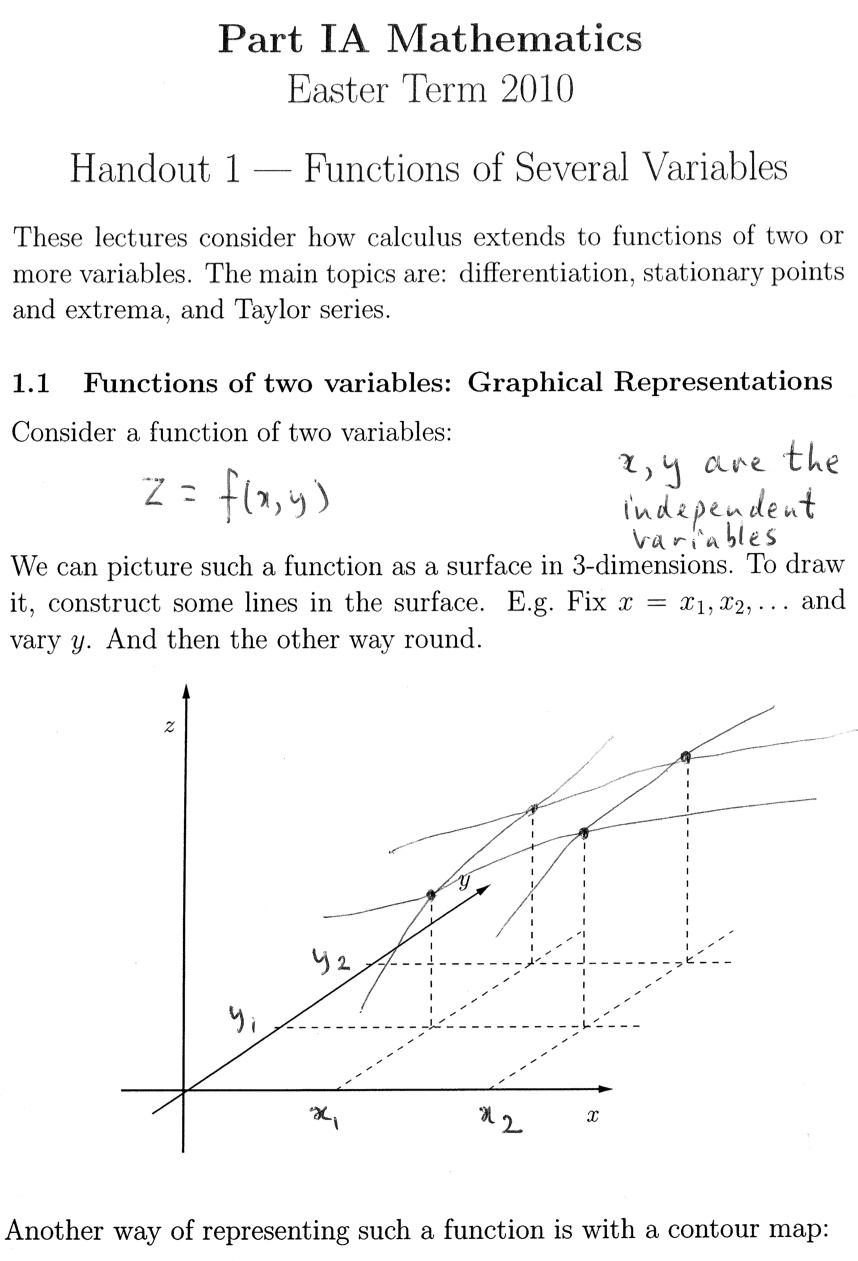
\includegraphics[width=\textwidth]{handout1.jpg}
    \end{subfigure}%
    \begin{subfigure}{.52\textwidth}
        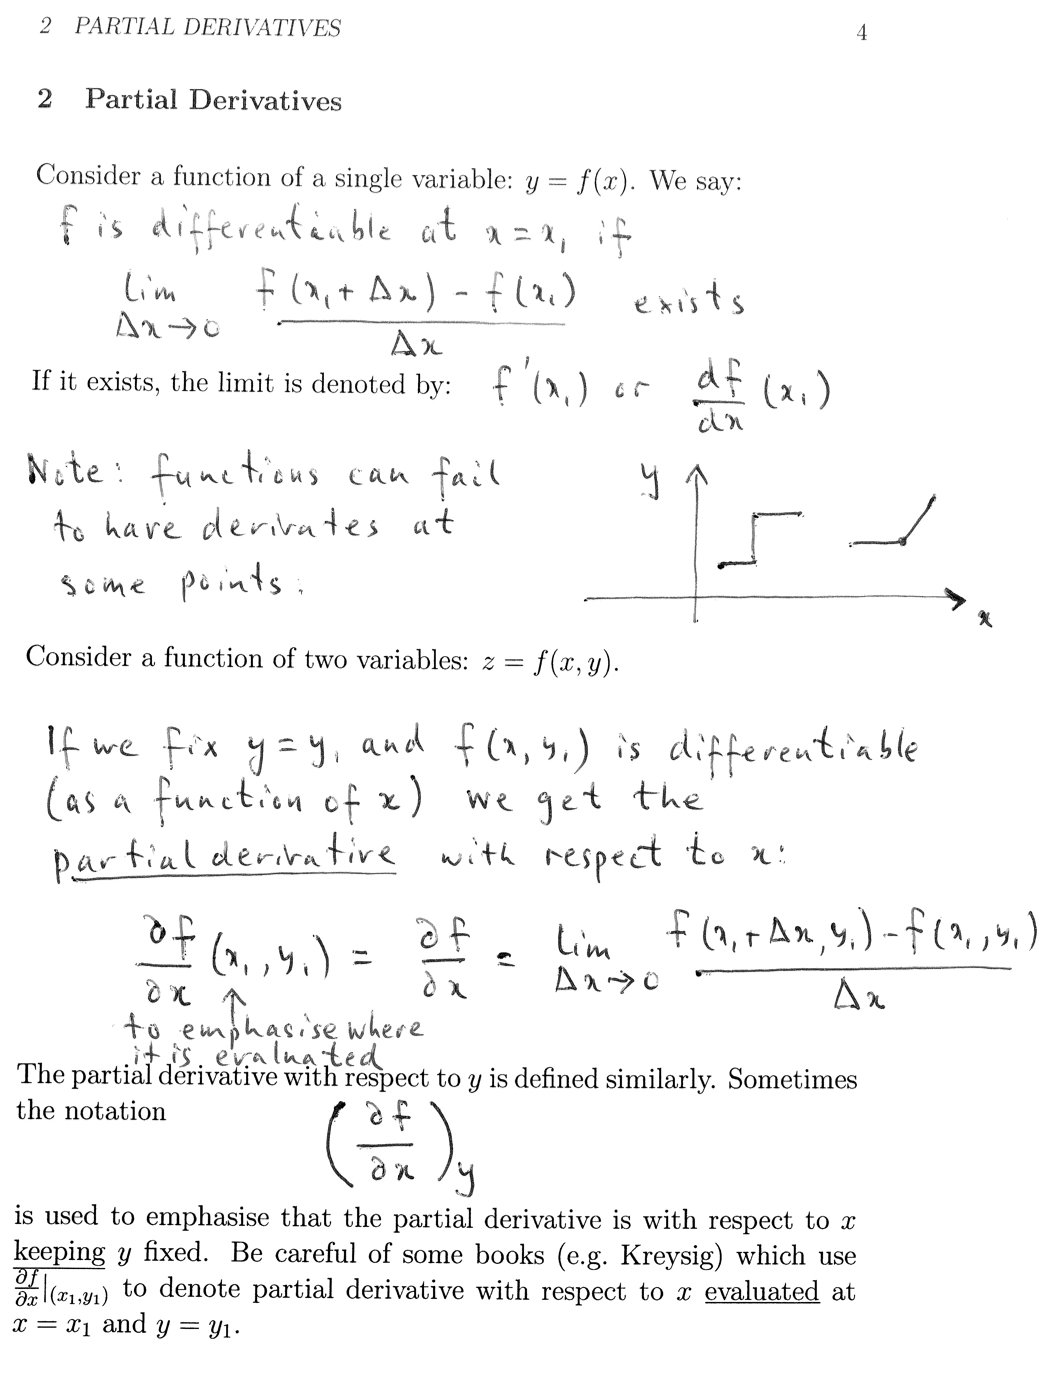
\includegraphics[width=\textwidth]{handout2.jpg}
    \end{subfigure}
    \caption{Examples of scanned handout pages with filled-in notes}
    \label{fig:intro-example-handouts}
\end{figure}

\begin{figure}[!htb]
    \centering
    \begin{subfigure}{.49\textwidth}
        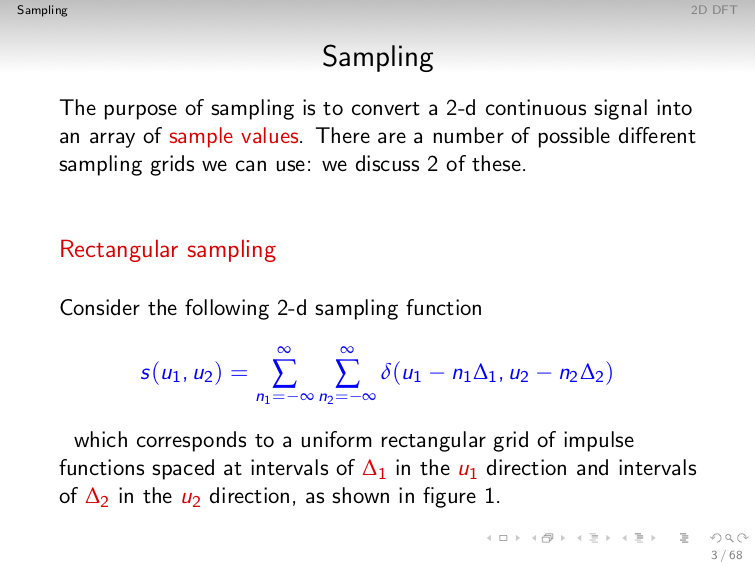
\includegraphics[width=\textwidth]{slide1.jpg}
    \end{subfigure}%
    \begin{subfigure}{.49\textwidth}
        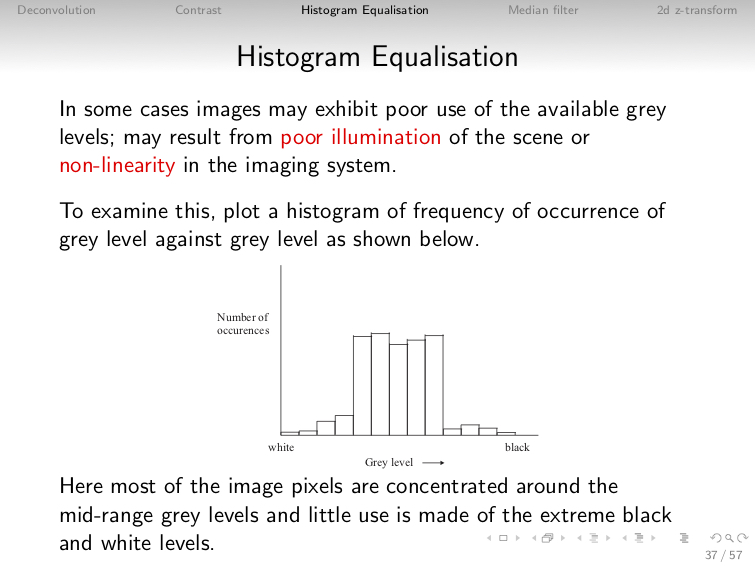
\includegraphics[width=\textwidth]{slide2.jpg}
    \end{subfigure}
    \caption{Examples of lecture slides typeset by \LaTeX}
    \label{fig:intro-example-slides}
\end{figure}


%%% Motivation %%%
\section{Motivation}

% situation
As mentioned in \Cref{sec:intro-background}, the Panopto service enables students to revisit parts of the lecture recordings, which has significantly enhanced their educational experience. A common situation for students is that they may have difficulties understanding specific parts in the handouts, such as the core concepts or some complicated equations, and they would like to refer back to lecturers' explanations to these parts. However, in order to find the correct parts of the lecture recordings that they are actually interested in, students still need to search back and forth in these recordings before they eventually arrive at the desired parts.

% ideal system
Therefore, it would be ideal to have a system which automatically analyses the lecture data (handouts + recordings) and brings us directly to the correct parts of the recordings upon selecting specific parts in the handouts. Such a system will aid the students to locate the desired parts of the recordings with minimum effort, and will even further improve their overall educational experience. The idea behind such a system is also termed as `talking handouts', which is the title of this project.

% reality
Unfortunately, few work has been done in designing and implementing such a system so there are not many useful references for this project. However, there are lots of relevant tools available such as OCR engines and speech recognisers, and it would still be interesting and worthwhile to try building a minimum working system based on these tools to test the feasibility of this idea, starting from the simplest assumptions.


%%% Project Aim
\section{Project Aims}
\label{sec:intro-aims}

% general aim
This project aims to investigate the feasibility of the idea `talking handouts' by designing, implementing and evaluating a minimum working software system which automatically computes the alignment (or mappings) between the chunks of handouts and the segments of the corresponding lecture recordings. Here we use the word `chunk' to denote a block of meaningful information in the handouts, and use the word `segment' to denote an interval with a starting time and an ending time in the lecture recordings. The wording `chunk' and `segment' will be used throughout the report.

% first subtask
The first major subtask of the project is to investigate methods of dividing the handouts into smaller chunks of information (at different scales) and extracting meaningful text from these chunks. A direct solution to this subtask is to use an OCR engine, which is adopted in the system design and further discussed in \Cref{chap:tess-ocr}.

% second subtask
The second major subtask of the project is to investigate speech-recognition based algorithms of aligning chunks of handouts with segments of lecture recordings. `Speech-recognition based' means that the lecture recordings are first fed into a speech recogniser and we use the output of the recogniser as one of the inputs of the alignment algorithm (the other input is the chunks of extracted handout text). The final system uses a \texttt{diff}-based alignment algorithm which is discussed in detail in \Cref{chap:align}.

% some assumptions
It would be worth mentioning that the project will only focus on handouts with filled-in handwritten notes (discussed in the first paragraph of \Cref{sec:intro-background}), since handouts of this type are fundamental to the CUED teaching (especially for Part IA and IB) and they also contain handwritten information which is interesting to investigate. 

In addition, the expression `speech-recognition based' in the second subtask has two further implications. The first implication is that the system is supposed to be using a mature speech recogniser and we are not going to care about how to tune the speech recogniser. The second implication is that we will only be using the audio information of the lecture recordings and the video information will be abandoned for simplicity. To avoid confusion, the wording `lecture audio file' is used instead of `lecture recording' in the rest of the report.

\section{Approach}

As a first step, basic assumptions are made on the system inputs and output. Based on these assumptions, the system architecture could then be designed. The 2 core subsystems, namely the OCR engine and the alignment algorithm, are investigated further to optimise the overall system performance, quantified by suitable metrics defined in the dedicated evaluation framework. Eventually, a GUI system is implemented to visualise the system alignment output and the results from the evaluation framework.

%%% Report Structure %%%
\section{Report Structure}

\begin{description}[leftmargin=5.5em,labelwidth=5em]
\item[Chapter 2] explains the basic assumptions on the system inputs and output
\item[Chapter 3] explains the design of the system architecture based on the basic assumptions in \Cref{chap:basic-assumptions} and briefly introduces the involved subsystems 
\item[Chapter 4] explains the Tesseract OCR engine with more detail, including the PLA and the training process
\item[Chapter 5] explains the mathematical formulation of the sequence alignment problem and how it is adapted to the actual alignment algorithm used in the system
\item[Chapter 6] explains the basic elements which support the operation of the system
\item[Chapter 7] explains how the system is evaluated
\item[Chapter 8] briefly introduces the setup of the actual software implementation
\item[Chapter 9] evaluates the system using the methodologies explained in \Cref{chap:eval-framework}
\item[Chapter 10] concludes the main findings and suggests possible future work
\end{description}


%% example nomenclatures
% \nomenclature[z-DKT]{DKT}{Draft Kiss Tumble}
% \nomenclature[z-PPC]{PPC}{Particles per cell}
\nomenclature[z-CUED]{CUED}{Cambridge University Engineering Department}
\nomenclature[z-VLE]{VLE}{Virtual Learning Environment}
\nomenclature[z-OCR]{OCR}{Optical Character Recognition}
%!TEX root = ../thesis.tex

%%%%% Chapter: Basic Assumptions %%%%%
\chapter{Basic Assumptions}

\ifpdf
    \graphicspath{{Chapter2/Figs/Raster/}{Chapter2/Figs/PDF/}{Chapter2/Figs/}}
\else
    \graphicspath{{Chapter2/Figs/Vector/}{Chapter2/Figs/}}
\fi


%%% Overview %%%
\section{Overview}

\Cref{fig:sys-diagram-basic} is a simplified diagram which shows the main inputs and output of the desired system. The system takes as inputs a handout file and its corresponding lecture audio file, and outputs the alignment result which maps each chunk of the handout to the corresponding segment (starting time + ending time) of the lecture audio file.

\begin{figure}[!hb]
  \centering
  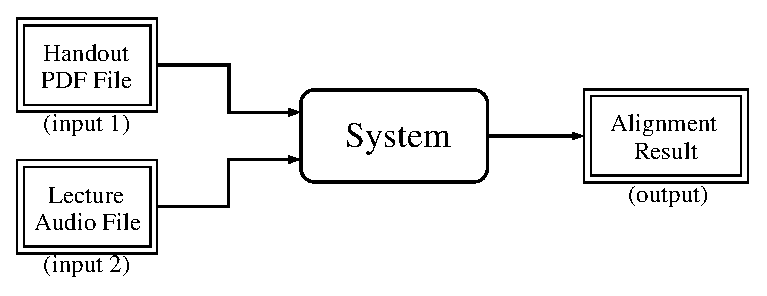
\includegraphics[width=.75\textwidth]{sys-diagram.eps}
  \caption{The inputs and output of the system}
  \label{fig:sys-diagram-basic}
\end{figure}

The handout files are assumed to be in PDF format, but the lecture audio files may take various formats. The alignment output is assumed to be taking the JSON format, which is readable by both human and computers. Additional assumptions on the inputs and output are discussed in the following sections.


%%% Handouts %%%
\section{Handouts}

The handouts are collections of necessary textual and figural information for the purpose of teaching specific courses, which form the crucial part of the system inputs. On Moodle (VLE), almost all uploaded handout files are in PDF format, so it's natural to restrict the input handout file of the system to be taking PDF format.

A proper model of the handouts is required for the purpose of designing the software system. At the first level of abstraction, a handout can be seen as a sequence of images. Each of the images could be further decomposed into basic components like text, equations, tables and figures. These components could be either handwritten or printed.

Since recognising complex components like equations, tables and figures could be really difficult and requires sophisticated algorithms, we will assume that the input handout files contain only text information (printed + handwritten) and will only focus on recognition of text.


%%% Lecture Audio Files %%%
\section{Lecture Audio Files}

The lecture audio file corresponding to the input handout PDF file is another important system input. The format of the input audio files are not particularly specified since we can convert the audio files into any desired format with a proper audio transcoder. Hence we will assume that the input audio files may take any audio format, with the only requirement that this format should be able to be transcoded to any required format in the system.

Another important assumption is made on how the lecturers deliver lectures. Normally, the lecturers will simply just read and explain handouts sequentially from top to bottom, page by page. However, they may occasionally skip sections or revisit previous sections during the lectures. In order to simplify the task in this project, we assume that the lecturers will refer to the handouts in strictly sequential order when giving lectures.


%%% Alignment Result %%%
\section{Alignment Results}

The eventual output of the software system is the alignment result which describes the matches between the chunks of the handout input and the segments of the associated audio file. Technically, any suitable form of text file could be used to describe the alignment result. In this project, the alignment output uses the JSON (JavaScript Object Notation) format since it's well strctured, completely human-readable and easily interpretable by computer programs.

\begin{figure}[!htb]
  \centering
  \begin{subfigure}{.45\textwidth}
    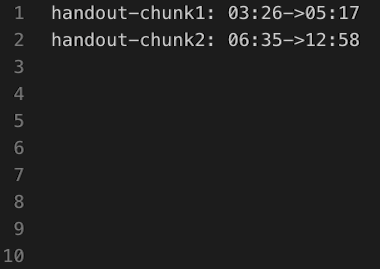
\includegraphics[width=\textwidth]{txt-example.png}
    \caption{Self defined format}
  \end{subfigure}
  \begin{subfigure}{.45\textwidth}
    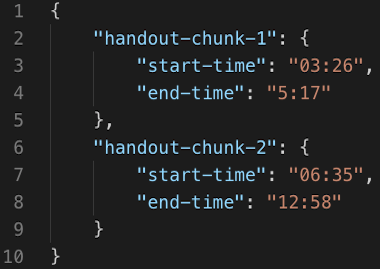
\includegraphics[width=\textwidth]{json-example.png}
    \caption{JSON format of the same information}
  \end{subfigure}
  \caption{Comparison between a self defined format and the JSON format which represent the same information}
  \label{fig:txt-json-compare}
\end{figure}

\Cref{fig:txt-json-compare} compares a piece of text of a self defined format with the JSON representation of the same information. We can notice that the JSON representation is longer but is organised in a more structured way. In addition, there are wide library supports for parsing JSON files in most of the mainstream programming languages (Java, Python, etc).



\nomenclature[z-PDF]{PDF}{Portable Document Format}
\nomenclature[z-JSON]{JSON}{JavaScript Object Notation}
%!TEX root = ../thesis.tex

%%%%% Chapter: System Architecture %%%%%
\chapter{System Architecture}


%%% Overview %%%
\section{Overview}


%% example of a nice-looking table
% \begin{table}
% \caption{Even better looking table using booktabs}
% \centering
% \label{table:good_table}
% \begin{tabular}{l c c c c}
% \toprule
% \multirow{2}{*}{Dental measurement} & \multicolumn{2}{c}{Species I} & \multicolumn{2}{c}{Species II} \\ 
% \cmidrule{2-5}
%   & mean & SD  & mean & SD  \\ 
% \midrule
% I1MD & 6.23 & 0.91 & 5.2  & 0.7  \\

% I1LL & 7.48 & 0.56 & 8.7  & 0.71 \\

% I2MD & 3.99 & 0.63 & 4.22 & 0.54 \\

% I2LL & 6.81 & 0.02 & 6.66 & 0.01 \\

% CMD & 13.47 & 0.09 & 10.55 & 0.05 \\

% CBL & 11.88 & 0.05 & 13.11 & 0.04\\ 
% \bottomrule
% \end{tabular}
% \end{table}

%!TEX root = ../thesis.tex

%%%%% Chapter: System Architecture %%%%%
\chapter{System Hyperparameters}

\ifpdf
    \graphicspath{{Chapter4/Figs/Raster/}{Chapter4/Figs/PDF/}{Chapter4/Figs/}}
\else
    \graphicspath{{Chapter4/Figs/Vector/}{Chapter4/Figs/}}
\fi


\section{Overview}


%%% Tesseract OCR %%%
\section{Tesseract OCR}

\subsection{Multi-scale Page Layout Analysis}

Recall that the Page Layout Analysis of the Tesseract OCR engine is able to identify distinct blocks (or bounding-boxes) of text by analysing the general layout of the input document. The Tesseract engine can provide different sets of bounding boxes at 5 scales: word, line, paragraph, block and page.

\Cref{fig:tess-pla-scales} shows the Tesseract output bounding-boxes at 4 different scales, excluding the `page' scale since the output of the `page' scale just contains one bounding-box which is the image boundary.

\begin{figure}[!htb]
  \centering
  \begin{subfigure}{.45\textwidth}
    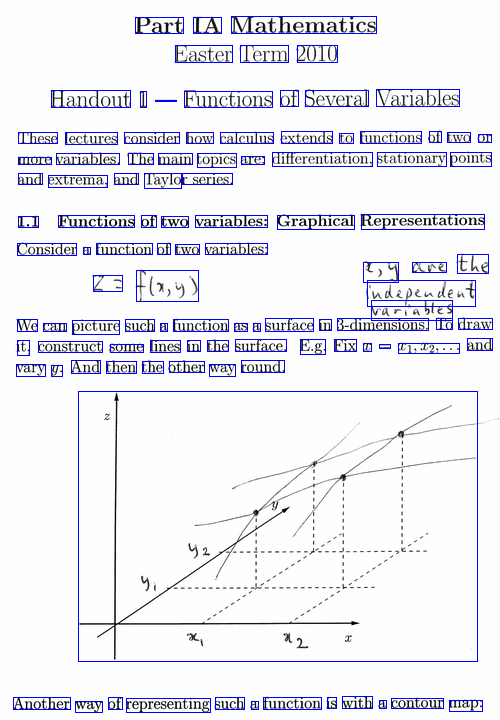
\includegraphics[width=\textwidth]{pla-word.png}
    \caption{Word scale}
  \end{subfigure}%
  \qquad
  \begin{subfigure}{.45\textwidth}
    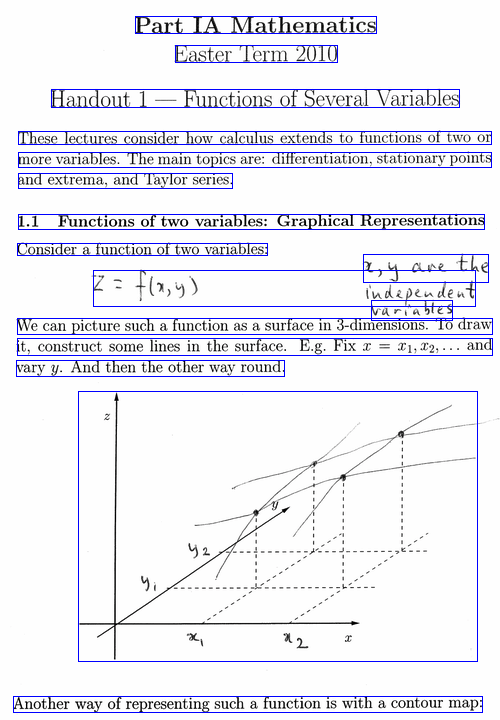
\includegraphics[width=\textwidth]{pla-line.png}
    \caption{Line scale}
  \end{subfigure}
  \vskip\baselineskip
  \begin{subfigure}{.45\textwidth}
    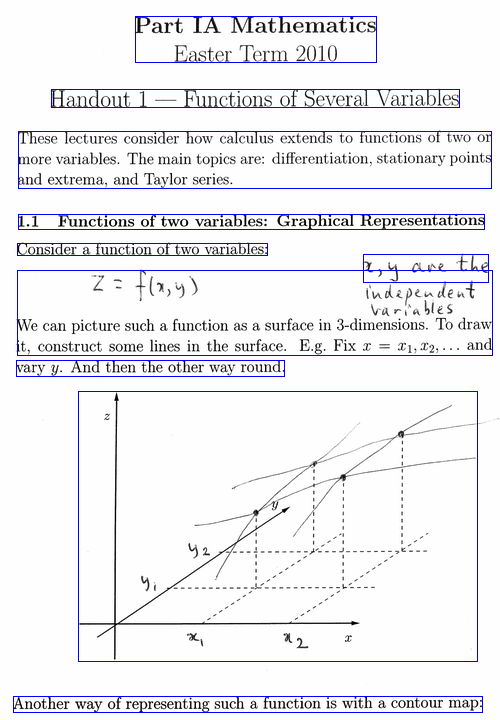
\includegraphics[width=\textwidth]{pla-par.png}
    \caption{Paragraph scale}
  \end{subfigure}%
  \qquad
  \begin{subfigure}{.45\textwidth}
    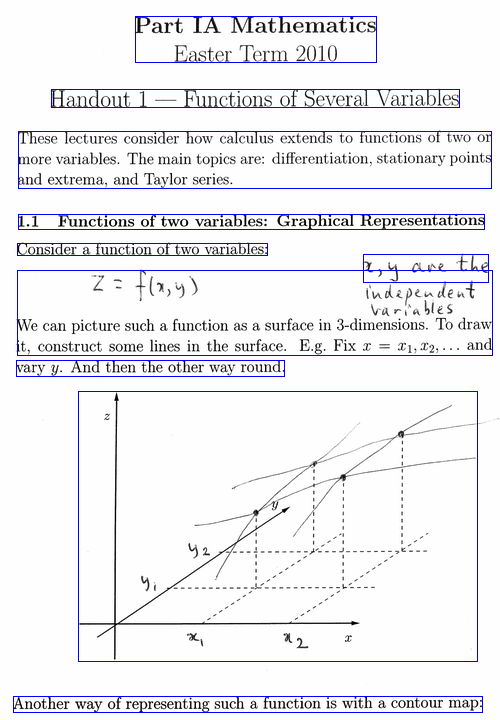
\includegraphics[width=\textwidth]{pla-block.png}
    \caption{Block scale}
  \end{subfigure}
  \caption{Different scales of Tesseract PLA}
  \label{fig:tess-pla-scales}
\end{figure}

In the actual system implementation, the user would be able to choose 4 different scales: word, line, paragraph and page. The `block' scale is removed from the implementation since in practice the difference between the `block' scale and the `paragraph' scale is negligible (which can be seen from \Cref{fig:tess-pla-scales}), and we keep the `paragraph' scale since the name `paragraph' is less ambiguous than `block'. 

We also keep the `page' scale in the system implementation for evaluation purposes described in later chapters, though this scale is not actually useful in practical use. The choice of PLA scale is considered to be one of the system hyperparameters.

\subsection{Model Switching}

Tesseract provides a large number of different models to support text recognition of different human languages. The default model is for recognising English text, which is named as \texttt{eng} in the Tesseract specification. 

Tesseract allows us to fine-tune existing models to produce improved models, or retrain from scratch to make completely new models. In this project, we have fine-tuned the default English model using additional handwritten data, and have included the fine-tuned model in the system implementation. The training of Tesseract OCR is further discussed in later chapters. 

Tesseract also allows us to specify what model to use before running the OCR engine. Using different models will eventually generate different recognition results. Therefore, the choice of the working Tesseract model is also one of the system hyperparameters.


\section{\texttt{diff}-based Alignment Algorithm}

\subsection{Problem Formulation}

Let $X$ = $X_1^n$ = ($X_1$,$X_2$,\ldots,$X_n$) and $Y$ = $Y_1^n$ = ($Y_1$,$Y_2$,\ldots,$Y_m$) be two sequences of symbols where $X_i \in A$ and $Y_j \in B$ for all $i$ and $j$. The sets $A$ and $B$ are also called \textit{alphabets}. Let $\phi$ be the `null symbol' which satisfies $\phi \notin A$ and $\phi \notin B$. Let $A^*$ = $A\cup\{\phi\}$ and $B^*$ = $B\cup\{\phi\}$.

Let $Z$ = $Z_1^p$ = ($Z_1$,$Z_2$,\ldots,$Z_p$), where $Z_i$ = $(S_i, T_i)$. Denote $S$ = $S_1^p$ = ($S_1$,$S_2$,\ldots,$S_p$) and $T$ = $T_1^p$ = ($T_1$,$T_2$,\ldots,$T_p$). We say $Z$ is an \textit{alignment} of sequences $X$ and $Y$ if:
\begin{enumerate}
  \item $Z_i \in A^* \times B^*$ and $Z_i \neq (\phi,\phi)$ for all $i$
  \item $X$ can be made equal to $S$ by inserting 0 or more null symbols $\phi$
  \item $Y$ can be made equal to $T$ by inserting 0 or more null symbols $\phi$
\end{enumerate}

Now define the Joint Weight Function, $\mathcal{F}(\cdot,\cdot)$: $A^* \times B^* \to \mathbb{R}$. The \textit{optimal alignment} $Z_{opt}$ is the alignment that maximise the sum of the joint weights, $\mathcal{W}$:
\begin{equation}
  Z_{opt} \,=\, \argmax_{Z} \mathcal{W}(Z) \,=\, \argmax_{Z} \sum_{i=1}^{p} \mathcal{F}(S_i,T_i)
\end{equation}
where $p$ denotes the length of $Z$ and may vary when $Z$ changes.

\subsection{Example: DNA Sequences}

In bioinformatics we often need to align different DNA sequences. To illustrate the above formulation, we use two example DNA sequences $X$ = \texttt{GCATGCT} and $Y$ = \texttt{GATTACA} with alphabets $A$ = $B$ = \{\texttt{A}, \texttt{T}, \texttt{G}, \texttt{C}\}. An example alignment could be:
\begin{center}
  \texttt{GCATG-CT}\\
  \texttt{G-ATTACA}
\end{center}
we can use $Z$ = (
  (\texttt{G},\texttt{G}),
  (\texttt{C},$\phi$),
  (\texttt{A},\texttt{A}),
  (\texttt{T},\texttt{T}),
  (\texttt{G},\texttt{T}),
  ($\phi$,\texttt{A}),
  (\texttt{C},\texttt{C}),
  (\texttt{T},\texttt{A})
) to express this alignment using the above formulation.

Usually when comparing two sequences, we care about the total weight (or score) of converting the first sequence to the second sequence by three basic operations: \textit{insertion}, \textit{deletion} and \textit{substitution}. These could be actually reflected in the Joint Weight Function $\mathcal{F}$:
\[
  \begin{cases}
    \mathcal{F}(\phi,y) & \text{\quad insert } y \text{ into } X \\
    \mathcal{F}(x,\phi) & \text{\quad delete } x \text{ from } X \\
    \mathcal{F}(x,y) & \text{\quad substitute } x \text{ with } y
  \end{cases}
\]
In the alignment of DNA sequences, it's common to assign positive scores for matches and negative scores for mismatches. If we define $\mathcal{F}(x,y)$ to be +1 if $x$ = $y$ and -1 otherwise, the total weight (or score) $\mathcal{W}$ can be calculated as:
\[ \mathcal{W}(Z) = 1 - 1 + 1 + 1 - 1 - 1 + 1 - 1 = 0 \]

\subsection{Alignment in the System}

In our system, we are working on 

\section{The Baseline System}



\nomenclature[z-JWF]{JWF}{Joint Weight Function}
%!TEX root = ../thesis.tex

%%%%% Chapter: System Architecture %%%%%
\chapter{Alignment Algorithm}
\label{chap:align}

\ifpdf
    \graphicspath{{Chapter5/Figs/Raster/}{Chapter5/Figs/PDF/}{Chapter5/Figs/}}
\else
    \graphicspath{{Chapter5/Figs/Vector/}{Chapter5/Figs/}}
\fi


\section{Overview}

The use of the \texttt{diff}-based alignment algorithm in the system is inspired by the work \cite{lanchantin2015development} which used a \texttt{diff}-based algorithm to align imperfect captions to audio of TV shows. In fact, the \texttt{diff} algorithm (which solves the LCS problem) is a subset of a more general mathematical formulation of the 2-sequence alignment problem, which will be explained in \Cref{sec:diff-formulation} with enough detail. After the discussion of the general formulation, we will explain how to adapt this formulation to the real alignment algorithm used in the system. 

\section{General Formulation of Alignment Problems}
\label{sec:diff-formulation}

Let $X$ = $X_1^n$ = ($X_1$,$X_2$,\ldots,$X_n$) and $Y$ = $Y_1^n$ = ($Y_1$,$Y_2$,\ldots,$Y_m$) be two sequences of symbols where $X_i \in A$ and $Y_j \in B$ for all $i$ and $j$. The sets $A$ and $B$ are also called \textit{alphabets}. Let $\phi$ be the \textit{null symbol} which satisfies $\phi \notin A$ and $\phi \notin B$. Let $A^*$ = $A\cup\{\phi\}$ and $B^*$ = $B\cup\{\phi\}$.

Let $Z$ = $Z_1^p$ = ($Z_1$,$Z_2$,\ldots,$Z_p$), where $Z_i$ = $(S_i, T_i)$. Denote $S$ = $S_1^p$ = ($S_1$,$S_2$,\ldots,$S_p$) and $T$ = $T_1^p$ = ($T_1$,$T_2$,\ldots,$T_p$). We say $Z$ is an \textit{alignment} of sequences $X$ and $Y$ if:
\begin{enumerate}
  \item $Z_i \in A^* \times B^*$ and $Z_i \neq (\phi,\phi)$ for all $i$
  \item $X$ can be made equal to $S$ by inserting 0 or more null symbols $\phi$
  \item $Y$ can be made equal to $T$ by inserting 0 or more null symbols $\phi$
\end{enumerate}

Now define the \textit{Joint Weight Function}, $\mathcal{F}(\cdot,\cdot)$: $A^* \times B^* \to \mathbb{R}$. The \textit{optimal alignment} $Z_{opt}$ is the alignment that maximise the sum of the joint weights, $\mathcal{W}$:
\begin{equation}
  Z_{opt} \,=\, \argmax_{Z} \mathcal{W}(Z) \,=\, \argmax_{Z} \sum_{i=1}^{p} \mathcal{F}(S_i,T_i)
\end{equation}
where $p$ denotes the length of $Z$ and may vary when $Z$ changes. The optimal alignment could be found by the \textit{Needleman-Wunsch Algorithm}~\cite{needleman1970general} with time and space complexity $O(nm)$.

\section{Example: DNA Sequences}

In bioinformatics we often need to align different DNA sequences. To illustrate the above formulation, we use two example DNA sequences $X$ = \texttt{GCATGCT} and $Y$ = \texttt{GATTACA} with alphabets $A$ = $B$ = \{\texttt{A}, \texttt{T}, \texttt{G}, \texttt{C}\}. An example alignment could be:
\begin{center}
  \texttt{GCATG-CT}\\
  \texttt{G-ATTACA}
\end{center}
we can use $Z$ = (
  (\texttt{G},\texttt{G}),
  (\texttt{C},$\phi$),
  (\texttt{A},\texttt{A}),
  (\texttt{T},\texttt{T}),
  (\texttt{G},\texttt{T}),
  ($\phi$,\texttt{A}),
  (\texttt{C},\texttt{C}),
  (\texttt{T},\texttt{A})
) to express this alignment using the formulation in \Cref{sec:diff-formulation}.

Usually when comparing two sequences, we care about the total weight (or score) of converting the first sequence to the second sequence by three basic operations: \textit{insertion}, \textit{deletion} and \textit{substitution}. These could be actually reflected in the Joint Weight Function $\mathcal{F}$:
\[
  \begin{cases}
    \mathcal{F}(\phi,y) & \text{\quad insert } y \text{ into } X \\
    \mathcal{F}(x,\phi) & \text{\quad delete } x \text{ from } X \\
    \mathcal{F}(x,y) & \text{\quad substitute } x \text{ with } y
  \end{cases}
\]
In the alignment of DNA sequences, it is common to assign positive scores for matches (same symbols) and negative scores for mismatches (insertions, deletions, substitutions with different symbols). If we define $\mathcal{F}(x,y)$ to be +1 if $x$ = $y$ and -1 otherwise, the total weight (or score) $\mathcal{W}$ can be calculated as:
\[ \mathcal{W}(Z) = + 1 - 1 + 1 + 1 - 1 - 1 + 1 - 1 = 0 \]

\section{Alignment in the System}
\label{sec:align-in-system}

In our system, we need to find the alignment between chunks of the handout text and segments of the lecture audio file. As a first step, we define $X$ to be the sequence of extracted words in the handout and define $Y$ to be the sequence of transcribed words in the corresponding audio file.

We can now define our Joint Weight Function $\mathcal{F}$. For the baseline alignment algorithm, the optimal alignment of $X$ and $Y$ just solves the \textit{longest common subsequence} problem, like the original \texttt{diff} algorithm. This is equivalent to using the following simple JWF:
\begin{equation}
  \mathcal{F}(x,y) = 
  \begin{cases}
    1 & \text{if } x = y\\
    0 & \text{otherwise}
  \end{cases}
  \label{eq:jwf-baseline}
\end{equation}
The optimal alignment $Z_{opt}$ could then be found with the JWF in \Cref{eq:jwf-baseline}.

As a next step, we should notice that each word in $X$ links to a unique chunk ID in the handout and each word in $Y$ is associated with a starting timestamp in the audio file. These information can be combined with the optimal alignment of $X$ and $Y$ to assign a time interval to each chunk of the handout.

\begin{figure}[!tb]
  \centering
  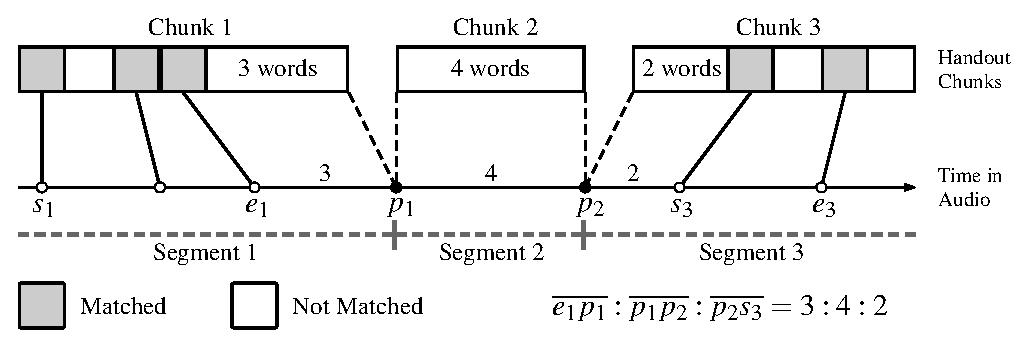
\includegraphics[width=.9\textwidth]{align-algo-fig.eps}
  \caption{Illustration of how to assign audio segments to handout chunks with the optimal alignment $Z_{opt}$}
  \label{fig:align-algo-fig}
\end{figure}

\Cref{fig:align-algo-fig} illustrates the strategy of assigning audio segments to handout chunks based on the optimal alignment $Z_{opt}$. The word matches in $Z_{opt}$ are indicated by solid lines between words in handout chunks and the points on the audio timeline. Chunk 1, 2, 3 have 3, 0, 2 matches respectively.

First we assign $\overline{s_1 e_1}$ and $\overline{s_3 e_3}$ to chunk 1 and chunk 3 respectively based on the matches. Then we divide $\overline{e_1 s_3}$ into three segments using two points $p_1$ and $p_2$ with ratio 3:4:2 based on these observations: there are 3 words between the last matched word and the last word in chunk 1; chunk 2 has no matches and has 4 words in total; there are 2 words between the first word and the first matched word in chunk 3. Finally, $p_1$ becomes the ending timestamp for chunk 1 and the starting timestamp for chunk 2, whilst $p_2$ becomes the ending timestamp for chunk 2 and the starting timestamp for chunk 3.

This strategy can be extended to any number of handout chunks. For each chunk with matches, the segment which corresponds to the first matched word and the last matched word is first assigned to this chunk. Then for each empty segment between the endpoints of the assigned segments, it is first divided into smaller segments based on the relative lengths (in number of words) of the unmatched words of the relevant handout chunks, and these smaller segments are then assigned to the corresponding chunks.

Note that this strategy is based on the assumption that the time spent on explaining a handout chunk is roughly proportional to the length of the chunk (in number of words).


\section{Extending the Baseline JWF}

Clearly the joint weight function can do more than just finding the longest common subsequence (\Cref{eq:jwf-baseline}) of two sequences. In this section we will discuss how the JWF could be extended in various ways.

\subsection{Adding Time Constraint}
\label{subsec:time-constraint}

Based on the assumptions that the lecturers will read the handouts in the strictly sequential order and that the amount of time spent on explaining a specific handout chunk is roughly proportional to the number of words in that chunk, we would expect that for any single match in the optimal alignment $Z_{opt}$, the difference between the relative position of the matching word in the handout and the relative position of the matching word in the audio file should be relatively small. 

Here we define the relative position of a word in the handout as the total number of its preceding words divided by the total number of words in the handout. Similarly we can define the the relative position of a word in the audio file to be the time difference between the timestamp of the word and the origin of the audio file, divided by the total length of the audio file. Clearly both of the relative positions range from 0 to 1.

In CUED the lectures are normally 50-minute long. Let $Z$ be a valid alignment and $(x,y)$ be an element in $Z$. Define $\mathcal{D}(x,y)$ as the difference between $x$'s relative position (in the handout) and $y$'s relative position (in the audio file) scaled by a factor of 50. We can interpret $\mathcal{D}(x,y)$ as the distance between $x$ and $y$ in minutes on the timeline of the audio file.

In the alignment algorithm, we would like to penalise large values of $\mathcal{D}(x,y)$. In the actual alignment system we use the Gaussian function with standard deviation $\sigma_t$, which yields the following JWF:
\begin{equation}
  \mathcal{F}(x,y) = 
  \begin{cases}
    \exp \left(-\frac{\mathcal{D}(x,y)}{2 \sigma_t^2}\right) & \text{if } x = y\\
    0 & \text{otherwise}
  \end{cases}
  \label{eq:jwf-gauss}
\end{equation}
we have removed the preceding normalising term of the Gaussian since it won't affect the optimal alignment. The Gaussian function decays when $\mathcal{D}(x,y)$ increases, which automatically penalises matches with large differences in relative positions.

\subsection{Penalising Common-word Matches}
\label{subsec:common-word-penalty}

In an alignment, matches of common words like `a', `the' and `it' should be assigned less weight than matches of other kinds of words. The Oxford Corpus have listed 100 most commonly used English words \cite{oec-common-words} based on the word frequencies in the corpus. Define the following function $\mathcal{C}(x)$ with a parameter $\alpha_c > 0$:
\begin{equation}
  \mathcal{C}(x) = 
  \begin{cases}
    \alpha_c & \text{if } x \text{ in the Oxford Corpus list}\\
    1 & \text{otherwise}
  \end{cases}
\end{equation}
Clearly $\alpha_c$ should be less than 1 in order to penalise common-word matches. Combining this function with \Cref{eq:jwf-gauss} yields the final JWF in the alignment algorithm:
\begin{equation}
  \mathcal{F}(x,y) = 
  \begin{cases}
    \mathcal{C}(x) \exp \left(-\frac{\mathcal{D}(x,y)}{2 \sigma_t^2}\right) & \text{if } x = y\\
    0 & \text{otherwise}
  \end{cases}
  \label{eq:jwf-final}
\end{equation}
note that the final $\mathcal{F}(x,y)$ has two adjustable parameters $\sigma_t$ and $\alpha_c$.


\nomenclature[z-JWF]{JWF}{Joint Weight Function}
\nomenclature[g-nullsymb]{$\phi$}{null symbol in sequence alignment}
\nomenclature[x-jwf]{$\mathcal{F}(x,y)$}{joint weight function with input symbols $x$ and $y$}
\nomenclature[x-sigma]{$\sigma_t$}{Gaussian standard deviation for adding time constraint}
\nomenclature[x-alpha]{$\alpha_c$}{coefficient for penalising common-word matches}
%!TEX root = ../thesis.tex

%%%%% Chapter: System Architecture %%%%%
\chapter{Basic Elements}
\label{chap:basic-elem}

\ifpdf
    \graphicspath{{Chapter6/Figs/Raster/}{Chapter6/Figs/PDF/}{Chapter6/Figs/}}
\else
    \graphicspath{{Chapter6/Figs/Vector/}{Chapter6/Figs/}}
\fi


\section{Overview}

Before introducing the evaluation framework and the software setup, we first need to explain the basic elements used in the system. Each of the basic elements is implemented as a Python class in the actual code. The definition of these basic elements forms the basis of the evaluation framework and the actual code implementation.

The basic elements are abstractions of the data in the system, and some of the elements are actually used as the inputs and outputs of the subsystems. The reason for placing the introduction of basic elements after introducing the inputs and outputs of the subsystems is that we try to avoid getting too technical at the very beginning and it would be easier to understand the basic elements after knowing roughly how the system works. 

\section{Elements Related to the OCR Engine}

\subsection{The BBox class}

The class name \texttt{BBox} stands for `bounding-box'. The \texttt{BBox} class defines the fundamental building block of the OCR output. An object of the \texttt{BBox} class contains a rectangle specified by the coordinates of the top-left and bottom-right corners, and also the enclosed text string. \Cref{fig:elem-bbox} shows an example \texttt{BBox} object. 

% bbox + bboxgroup
\begin{figure}[ht]
    \centering
    \begin{subfigure}[t]{0.48\textwidth}
        \centering
        
\includegraphics[width=\textwidth]{elem-bbox.eps}
        \caption{A \texttt{BBox} object}
        \label{fig:elem-bbox}
    \end{subfigure}%
    ~ 
    \begin{subfigure}[t]{0.48\textwidth}
        \centering
        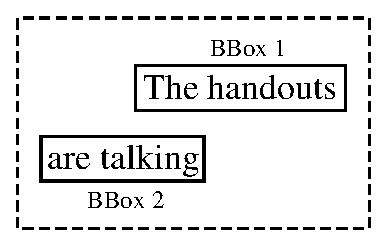
\includegraphics[width=\textwidth]{elem-bboxgroup.eps}
        \caption{A \texttt{BBoxGroup} object}
        \label{fig:elem-bboxgroup}
    \end{subfigure}
    \caption{Examples of \texttt{BBox} and \texttt{BBoxGroup} objects}
\end{figure}

\subsection{The BBoxGroup class}

A \texttt{BBoxGroup} object is simply a collection of \texttt{BBox} objects. Usually the \texttt{BBox} objects contained in a \texttt{BBoxGroup} object are closely related to each other, for example a sentence across multiple lines can be expressed as a \texttt{BBoxGroup} object. \Cref{fig:elem-bboxgroup} shows an example \texttt{BBoxGroup} object.

The \texttt{BBoxGroup} class defines the atomic level of alignment input at the OCR side. The single mapping from a \texttt{BBoxGroup} object to the corresponding parts of the audio file cannot be further divided.

\subsection{The BBoxGroups class}

As the class name suggests, a \texttt{BBoxGroups} object is simply a collection of \texttt{BBoxGroup} objects. In the actual implementation, the \texttt{BBoxGroups} class inherits from the Python's built-in \texttt{list} class, and hence a \texttt{BBoxGroups} object has all the properties of Python lists.

The output of the OCR engine is a \texttt{BBoxGroups} object, which is a list of atomic objects for the alignment process. 

\section{Elements Related to the Speech Recogniser}

\subsection{The TStamp class}

A \texttt{TStamp} object represents a timestamp in the audio file. The class defines three attributes: \texttt{min} (minutes), \texttt{sec} (seconds, within range [0, 59]) and \texttt{msec} (milliseconds, within range [0, 999]).

\subsection{The TInterval class}

A \texttt{TInterval} object represents an interval in the audio file which consists of two \texttt{TStamp} objects, indicating the starting timestamp and the ending timestamp respectively. This class provides an straightforward way of representing segments of the audio file.

\subsection{The WStamp class}

The class name \texttt{WStamp} stands for `word with a timestamp'. A \texttt{WStamp} object represents a recognised word and the associated starting timestamp as in the input audio file. This class forms the basis of the speech recogniser output, which is also called the transcript of the audio file. 

\subsection{The WStamps class}

A \texttt{WStamps} object is a collection of multiple \texttt{WStamp} objects. Similar to the \texttt{BBoxGroups} class, the \texttt{WStamps} class also inherits from the Python built-in \texttt{list} class.

This class can be used to describe the speech recogniser output (also called the `transcript'). In the actual system implementation, the output of the speech recogniser is just a \texttt{WStamps} object.

\section{Elements Related to the Alignment Algorithm}

\subsection{The TIntervalGroup class}

A \texttt{TIntervalGroup} object is a collection of multiple \texttt{TInterval} objects. In the final alignment result, each \texttt{BBoxGroup} object uniquely matches a \texttt{TIntervalGroup} object. Hence, the \texttt{TIntervalGroup} class is a fundamental part of the alignment result.

\subsection{The Match class}

A \texttt{Match} object simply represents a single match in the alignment result, which consists of a {BBoxGroup} object and a \texttt{TIntervalGroup} object. 

\subsection{The Matches class}
\label{sec:basic-elem-matches}

A \texttt{Matches} object is a collection of multiple \texttt{Match} objects. This class also inherits from the Python built-in \texttt{list} class. In the actual implementation, the final alignment result is a \texttt{Matches} object. \Cref{fig:elem-matches} shows the relationships between different classes, starting from a \texttt{Matches} object.

\begin{figure}[!htb]
    \centering
    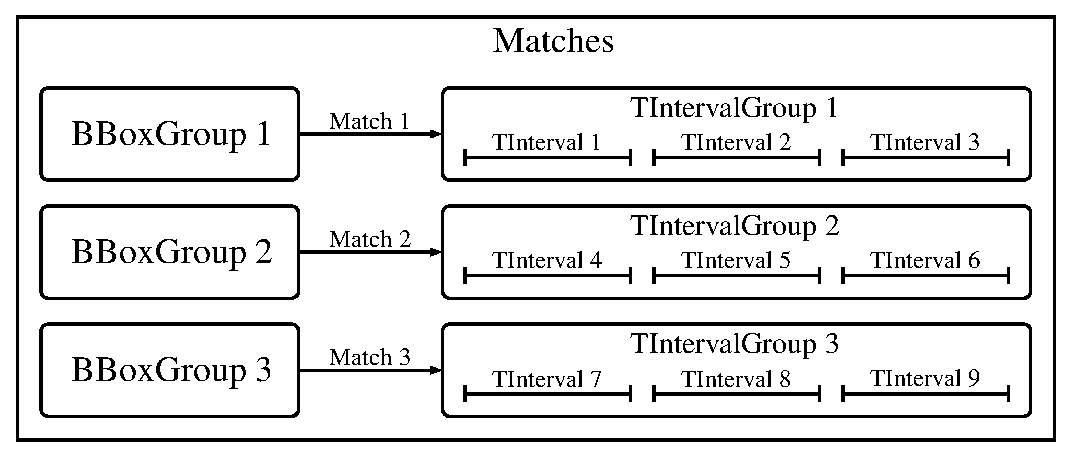
\includegraphics[width=0.9\textwidth]{elem-matches.eps}
    \caption{Relationships between different classes inside a \texttt{Matches} object}
    \label{fig:elem-matches}
\end{figure}

\section{System Architecture Revisited}

We shall now revisit the system architecture based on the knowledge of the basic element definitions. \Cref{fig:elem-sys-diagram} shows the updated diagram labelled with the defined classes of the basic elements.

\begin{figure}[!htb]
    \centering
    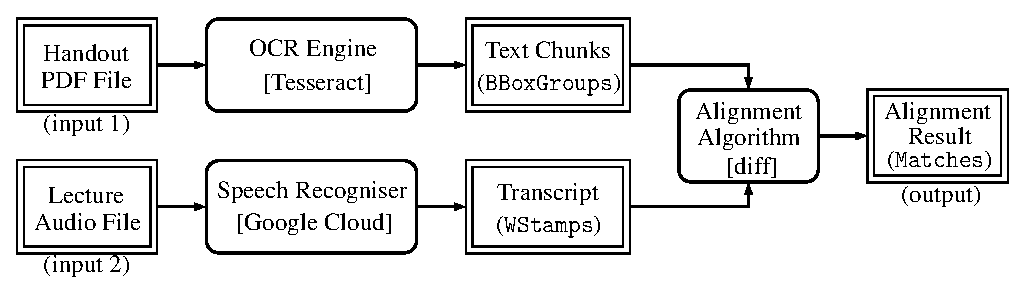
\includegraphics[width=0.95\textwidth]{elem-sys-diagram.eps}
    \caption{Basic elements as inputs / outputs within the system}
    \label{fig:elem-sys-diagram}
\end{figure}
%!TEX root = ../thesis.tex

%%%%% Chapter: System Evaluation %%%%%
\chapter{Evaluation Framework}
\label{chap:eval-framework}

\ifpdf
    \graphicspath{{Chapter7/Figs/Raster/}{Chapter7/Figs/PDF/}{Chapter7/Figs/}}
\else
    \graphicspath{{Chapter7/Figs/Vector/}{Chapter7/Figs/}}
\fi


\section{Overview}

\section{The Ground-Truth Data}

The ground-truth (GT) data of a single set of input lecture data (a handout PDF file + its associated audio file) can be seen as the correct mappings from the handout chunks (\texttt{BBoxGroup} objects) to the corresponding parts of the audio file (\texttt{TIntervalGroup} objects). The ground truth data as a whole can be represented by a \texttt{Matches} object described in \Cref{sec:basic-elem-matches}.

The ground-truth data should be labelled at the finest spatial scale possible, which means each \texttt{BBoxGroup} object in the ground-truth data is supposed to be as small (in its total area) as possible. This ensures the feasibility of the multi-scale evaluation of the alignment algorithm.

\section{Evaluating the OCR PLA}

Recall that the page layout analysis (PLA) of the Tesseract OCR engine produces a set of bounding-boxes which identifies distinct text regions in the PDF input. In \Cref{fig:eval-ocr-pla}, we can see how true positives (TP), true negatives (TN), false positives (FP) and false negatives (FN) are identified, given the bounding-boxes (a \texttt{BBoxGroups} object as a whole) in the ground-truth data. Here we assume that the bounding-boxes are non-overlapping for the ground-truth data and the OCR output respectively (in practice the OCR output bounding-boxes may overlap a little bit).

\begin{figure}[!htb]
    \centering
    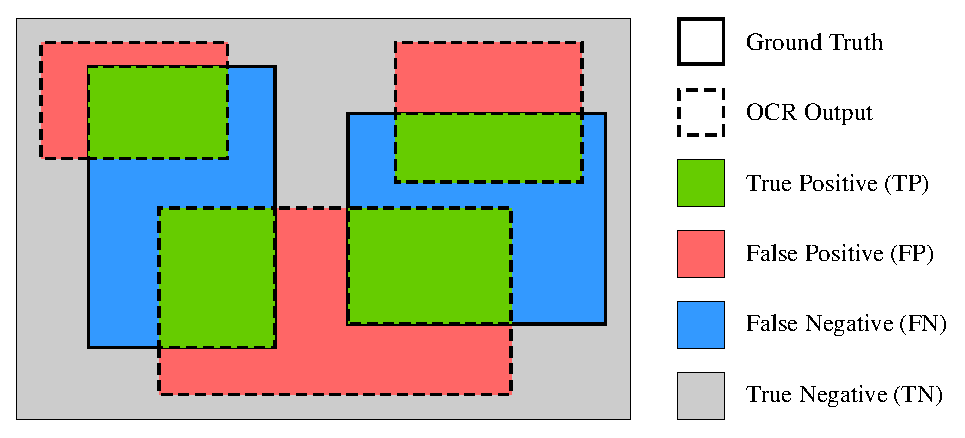
\includegraphics[width=0.75\textwidth]{eval-ocr-pla.eps}
    \caption{TP, TN, FP and FN in the evaluation of PLA}
    \label{fig:eval-ocr-pla}
\end{figure}

The key evaluation metrics are the \textit{true positive rate} (TPR) and \textit{true negative rate} (TNR), which are calculated as follows:
\[
    \begin{cases}
        \text{TPR \,=\, TP / (TP + FN)} \\
        \text{TNR =\, TN / (TN + FP)}
    \end{cases}
\]
Note that TPR is also called the recall rate. To calculate TPR and TNR, we sum up all rectangle areas for each certain type (TP, TN, FP and FN) and then substitute the values into the above equations.

The TPR (recall rate) essentially measures the fraction of the intersection area between the OCR output bounding-boxes and the bounding-boxes of the ground-truth data, with respect to the total area of the ground-truth bounding-boxes. The TNR, on the other hand, reflects the fraction of area which is correctly identified as negative. A low TNR value means that we have too much false positive area (or a high False Positive Rate) in the OCR output. Clearly both TPR and TNR should be maximised.


\section{Evaluating the OCR Text Recognition}

The text recognition accuracy of the Tesseract OCR engine is measured by the \textit{word error rate} (WER). Let $X$ be the concatenation of all words in the OCR recognition result (a \texttt{BBoxGroups} object) and let $Y$ be the concatenation of all words in the \texttt{BBoxGroup} objects of the ground-truth data (recall that the ground-truth data as a whole is a \texttt{Matches} object). We first obtain the optimal alignment $Z_{opt}$ of $X$ and $Y$ using the following joint weight function:
\begin{equation}
    \mathcal{F}(x,y) = 
    \begin{cases}
        0 & x = y \text{ (match)} \\
        -4 & x = \phi \text{ (insertion) or } y = \phi \text{ (deletion)} \\
        -6 & x \neq y \neq \phi \text{ (substitution)}
    \end{cases}
\end{equation}
The weight ratio of insertion, deletion and substitution is defined as 4:4:6 since we want a single substitution to cost more than a single insertion or substitution, but cost less than an insertion plus a substitution. 

Let $I$, $D$ and $S$ be the numbers of insertions, deletions and substitutions in the optimal alignment $Z_{opt}$. Then the WER of OCR text recognition is calculates as:
\begin{equation}
    \text{WER} = \frac{I + D + S}{N}
\end{equation}
where $N$ is the length of the reference string $Y$ (ground-truth).


\section{Evaluating the Alignment Algorithm}

Evaluation of the alignment algorithm is more difficult since the scale of the OCR output bounding-boxes (a \texttt{BBoxGroups} object as a whole) may vary. We first need to find the correct ground-truth audio segments (\texttt{TIntervalGroup} object) for each bounding-box (at different scales) of the OCR output, and then compare the segments from the output of the alignment algorithm with the correct segments in the time domain. 

\subsection{Handling Multiple Scales}

Let's start with an example. \Cref{fig:eval-align-scale} shows 3 different OCR output bounding-boxes of various scales (in 3 different colors other than black) and their assigned ground-truth audio segments. The ground-truth bounding-boxes (\texttt{BBoxGroup} objects) and their matching audio segments (\texttt{TIntervalGroup} objects) are shown in black. 

\begin{figure}[!tb]
    \centering
    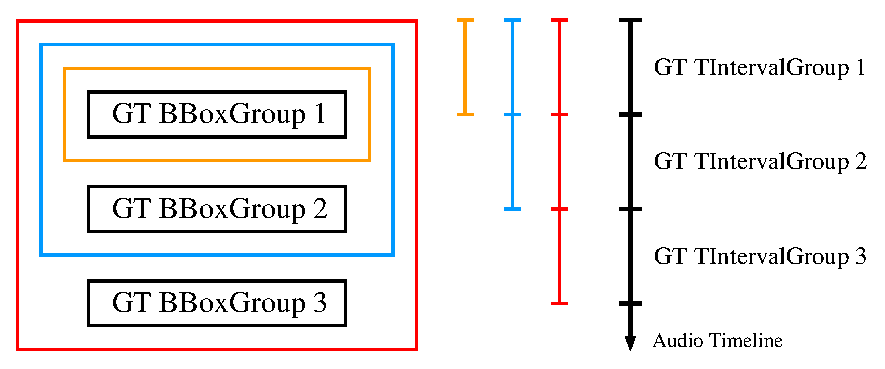
\includegraphics[width=.8\textwidth]{eval-align-scale.eps}
    \caption{Relationship between the scale of the bounding-box and its assigned ground-truth audio segments}
    \label{fig:eval-align-scale}
\end{figure}

It's clear that the number of assigned ground-truth audio segments generally increases with the bounding-box scale. For example in \Cref{fig:eval-align-scale}, the yellow bounding-box encloses only the first \texttt{BBoxGroup} object and is assigned just the first ground-truth audio segment, while the red bounding-box includes all the \texttt{BBoxGroup} objects so it is assigned all three audio segments.

However, a ground-truth \texttt{BBoxGroup} object may not necessarily be perfectly enclosed in an OCR output bounding-box. Often the ground-truth bounding-box is partially enclosed by multiple OCR bounding-boxes, in which case we need to decide which OCR bounding-box the ground-truth bounding-box belongs to.

\begin{figure}[!htb]
    \centering
    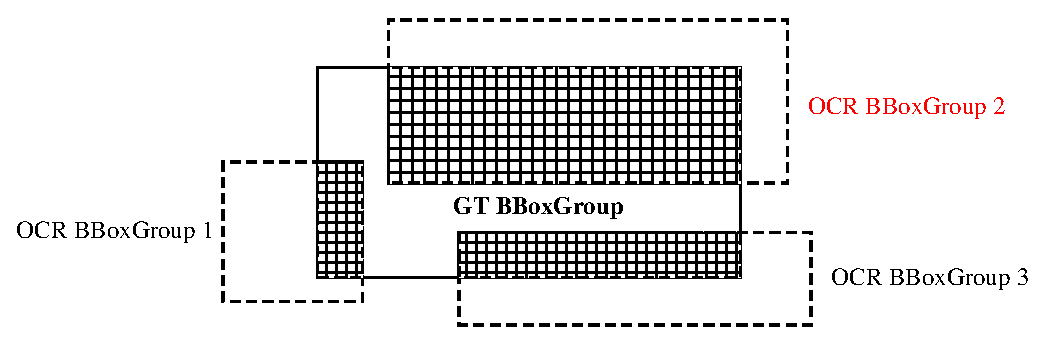
\includegraphics[width=.8\textwidth]{eval-gt-assign.eps}
    \caption{Strategy of GT bounding-box assignment to OCR boxes}
    \label{fig:eval-gt-assign}
\end{figure}

In this evaluation framework we use a very simple strategy which assigns each ground-truth \texttt{BBoxGroup} object to the OCR \texttt{BBoxGroup} object which has the largest intersection area with this ground-truth \texttt{BBoxGroup} object. \Cref{fig:eval-gt-assign} shows an example GT \texttt{BBoxGroup} object intersecting 3 OCR \texttt{BBoxGroup} objects, and it is assigned to OCR \texttt{BBoxGroup} 2 since they have the largest intersection area.

\subsection{Time-Domain Alignment Evaluation}

\begin{figure}[!tb]
    \centering
    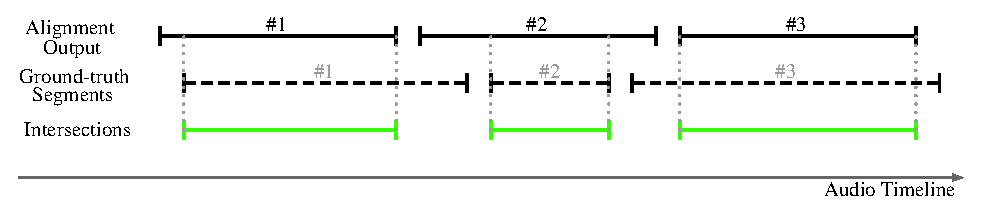
\includegraphics[width=.9\textwidth]{eval-time-domain.eps}
    \caption{Comparing multiple audio segments on a single timeline}
    \label{fig:eval-time-domain}
\end{figure}

After the ground-truth assignment in the previous section, for each OCR output bounding-box we concatenate the assigned ground-truth audio segments (\texttt{TIntervalGroup} objects) in the time domain, and compare the GT segments with the alignment output segments corresponding to the OCR bounding-box. \Cref{fig:eval-time-domain} shows 3 sets of alignment output segments, their corresponding GT segments (dashed) and the intersections between the alignment segments and the GT segments (in green). We then define the recall rate of alignment in time domain:
\begin{equation}
    \text{Alignment Recall Rate}\,=\,\frac{\text{Total length of intersections}}{\text{Total length of the GT segments}}
\end{equation}
which is the evaluation metric for the alignment accuracy in time domain.


\nomenclature[z-GT]{GT}{Ground Truth}
\nomenclature[z-TPR]{TPR}{True Positive Rate}
\nomenclature[z-TNR]{TNR}{True Negative Rate}
%!TEX root = ../thesis.tex

%%%%% Chapter: Software Setup %%%%%
\chapter{Software Setup}

\ifpdf
    \graphicspath{{Chapter8/Figs/Raster/}{Chapter8/Figs/PDF/}{Chapter8/Figs/}}
\else
    \graphicspath{{Chapter8/Figs/Vector/}{Chapter8/Figs/}}
\fi


\section{Overview}

\DTsetlength{0.2em}{6em}{0.2em}{0.7pt}{2.3pt}

A simplified directory tree of the source code is shown below:

\dirtree{%
.1 root/.
.2 system/.
.3 aux/.
.3 elements/.
.3 subsystems/.
.2 eval/.
.3 align.py.
.3 ocr.py.
.2 gui/.
.3 root.py.
.3 system.py.
.3 labeller.py.
}

The \texttt{system/} folder contains the fundamental setups including the implementations of all the subsystems (OCR, Speech Recogniser, Alignment Algorithm), all the basic elements explained in \Cref{chap:basic-elem} and some auxilliary functions like the \texttt{diff} with JWF input. The \texttt{eval/} folder contains functions to compute all the evaluation metrics described in \Cref{chap:eval-framework}. The \texttt{gui/} folder visualises the main functionalities implemented in the \texttt{system/} and \texttt{eval/} folders.

\section{The \texttt{system/} Folder}

The \texttt{system/} folder implements the core parts of the system architecture, which forms the basis of the entire software setup. The \texttt{system/} folder contains 3 main child folders: \texttt{subsystems/}, \texttt{elements/} and \texttt{aux/}.

\subsection{The \texttt{subsystems/} child folder}

The \texttt{subsystems/} child folder contains the implementations (or wrappers) of the Tesseract OCR engine, Google Cloud Speech Recogniser and the \texttt{diff}-based alignment algorithm, as 3 separate Python (\texttt{.py}) files (not shown in the directory tree for simplicity).

The Tesseract OCR is integrated into the system using the \texttt{pytesseract} wrapper, and the engine can run locally without Internet connection. The Google Cloud Speech-to-Text service also has Python APIs, but it requires stable Internet connection to send requests and receive the transcription results. The Google Cloud also needs my personal credentials before the speech-to-text service can actually be used in the system.

The \texttt{diff}-based alignment algorithm is based on the self-implemented JWF-based alignment algorithm stored in the \texttt{aux/} folder. It first obtain the optimal alignment based on the parameterised JWF function defined in \Cref{eq:jwf-final}, and then return the final alignment result as a \texttt{Matches} object using the method explained in \Cref{sec:align-in-system}.

\subsection{The \texttt{elements/} child folder}

This child folder contains all the implementations of the basic elements defined in \Cref{chap:basic-elem}. This folder is a core dependency for almost all other files, especially for the files in the \texttt{system/} and the \texttt{eval/} folder.

\subsection{The \texttt{aux/} child folder}

This child folder includes the helper functions used by the system. We have mentioned earlier that this folder contains an important implementation which solves the optimal alignment of two sequences with a configurable JWF input. The actual implementation of finding the optimal alignment uses the Hirschberg's algorithm \cite{hirschberg1975linear}, which can achieve linear space complexity by a clever modification of the Needleman-Wunsch Algorithm (mentioned in \Cref{sec:diff-formulation}).


\section{The \texttt{eval/} Folder}

The \texttt{eval/} folder contains two main files \texttt{ocr.py} and \texttt{align.py}, which implement the evaluation functions for the Tesseract OCR and the alignment algorithm respectively. These evaluation functions highly rely on the basic elements and their associated operations defined in \texttt{system/elements/}. For instance, the intersection area between two \texttt{BBoxGroup} objects \texttt{a} and \texttt{b} could be calculated using the simple expression \texttt{(a \& b)}, which is heavily used in the evaluation of OCR output bounding-boxes.


\section{The \texttt{gui/} Folder}

The GUI implementation visualises the core components in the system, including the system parameter control, final system output and the system evaluation results. The GUI implementation is based on the Tkinter module, which is the Python binding to the Tk GUI Toolkit. It allows the users to easily interact with the core system (implemented in \texttt{gui/system.py}), and also allows the system developers (like me) to label the ground-truth dataset for the purpose of evaluation (implemented in \texttt{gui/labeller.py}). The GUI can be initiated by running \texttt{gui/root.py}.

\subsection{\texttt{gui/system.py}}

\begin{figure}[!ht]
    \centering
    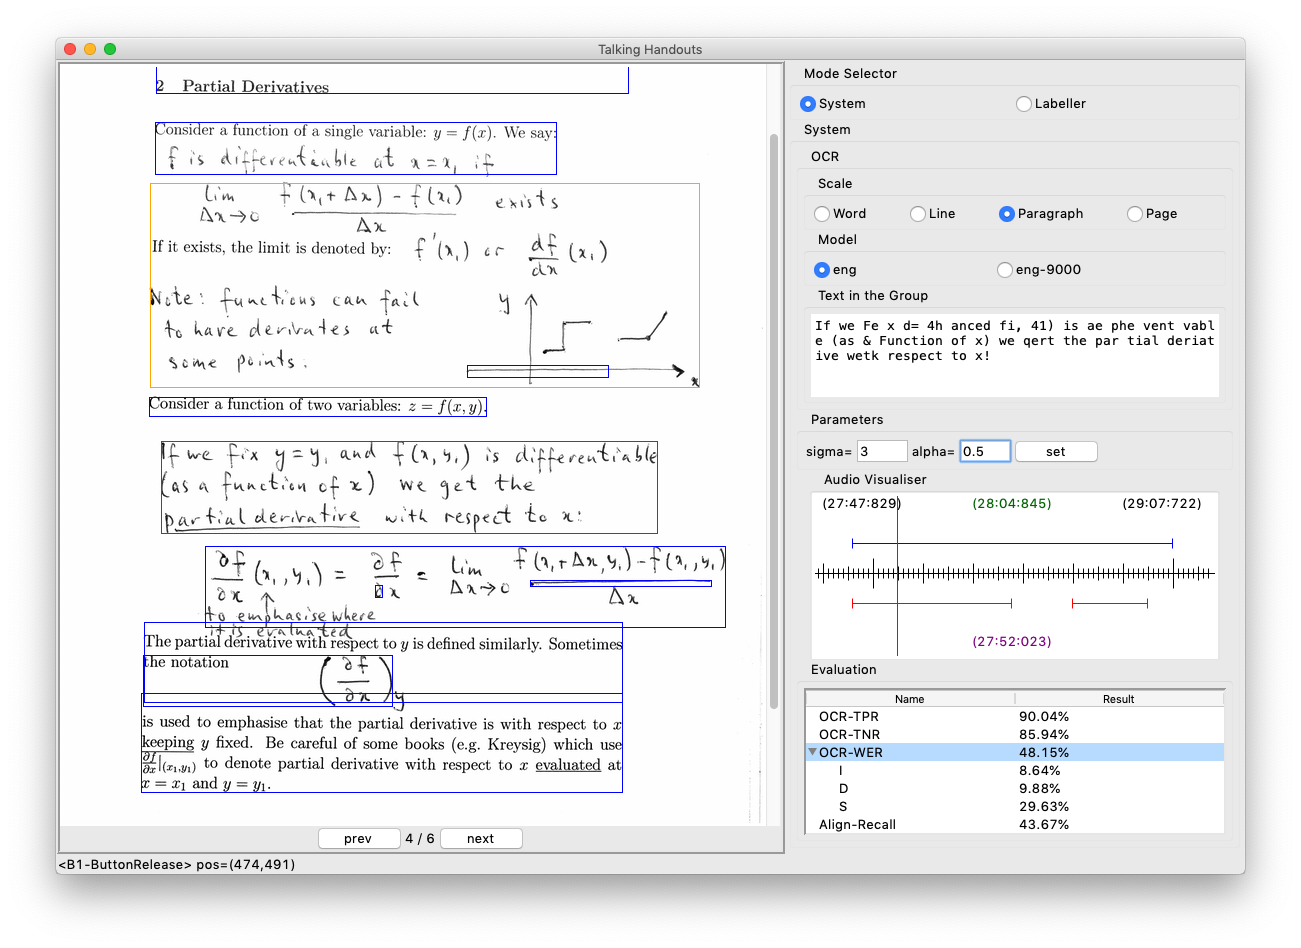
\includegraphics[width=\textwidth]{gui-system.png}
    \caption{The `System' mode of the GUI}
    \label{fig:gui-system}
\end{figure}

\Cref{fig:gui-system} shows a screenshot of the `system' mode of the GUI. The users are able to select between the 4 OCR scales, 2 OCR models (\texttt{eng} and \texttt{eng-9000}) and they could also adjust the parameters $\sigma_t$ and $\alpha_c$ for the alignment algorithm. The resulting bounding-boxes are rendered in the left, and the corresponding alignment output audio segments (in blue) and the assigned ground-truth segments (in red) are shown in the audio visualiser to the right.

Users can click any bounding-box in the left and listen to the lecture audio by clicking a specific position in the audio visualiser. The audio playback can be stopped by pressing spacebar. The evaluation results are listed in the bottom-right corner.

\subsection{\texttt{gui/labeller.py}}

\begin{figure}[!ht]
    \centering
    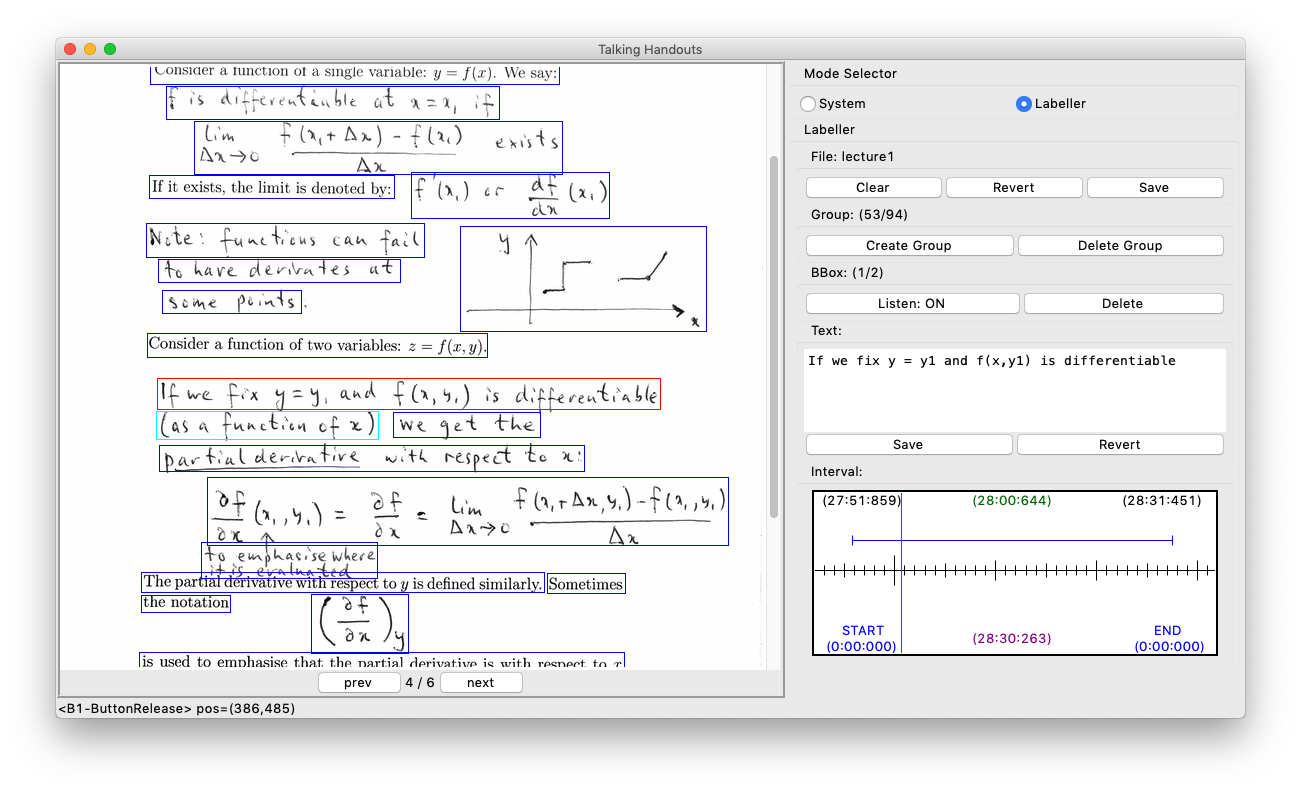
\includegraphics[width=.9\textwidth]{gui-labeller.png}
    \caption{The `Labeller' mode of the GUI}
    \label{fig:gui-labeller}
\end{figure}

The `labeller' mode is implemented for the purpose of labelling ground-truth data for the evaluation framework. A new \texttt{BBoxGroup} object can be created by clicking `Create Group' and \texttt{BBox} objects can be added to this group by drawing rectangles directly in the left on the handouts. The reference text for each \texttt{BBox} should be typed in the textbox above the audio visualiser. For each labelled \texttt{BBoxGroup}, the corresponding audio segments can also be labelled in the audio visualiser on the right.
%!TEX root = ../thesis.tex

%%%%% Chapter: Software Setup %%%%%
\chapter{Evaluation Results}
\label{chap:eval-results}

\ifpdf
    \graphicspath{{Chapter9/Figs/Raster/}{Chapter9/Figs/PDF/}{Chapter9/Figs/}}
\else
    \graphicspath{{Chapter9/Figs/Vector/}{Chapter9/Figs/}}
\fi


\section{Overview}

\begin{table}[!htb]
    \caption{Adjustable System Parameters}
    \centering
    \label{tab:sys-param-list}
    \begin{tabular}{l l c}
    \toprule
    Name & Description & Range \\
    \midrule
    OCR-scale & Scale of the OCR PLA & \{`word', `line', `paragraph', `page'\} \\
    OCR-model & OCR model used for recognition & \{`\texttt{eng}', `\texttt{eng-9000}'\} \\
    JWF-$\sigma_t$ & Gaussian STD for time constraint & (0, $\infty$) \\
    JWF-$\alpha_c$ & Penalty for common words & (0, 1]\\
    \bottomrule
    \end{tabular}
\end{table}

A number of parameters in the system can be adjusted. \Cref{tab:sys-param-list} lists all the adjustable system parameters. Evaluation can be performed on the system with various sets of parameters.

Due to the time limitation and the high complexity of labelling the ground-truth data for lectures, only a single set of ground-truth data has been labelled for the system evaluation. The labelled ground-truth data corresponds to the first hour-long lecture of Part IA Math (2010) taught by Prof. Malcolm Smith.

The methodology of evaluation is simple: starting from a set of baseline parameters, we try to adjust each parameter individually in turn and observe the effects. Then we combine the individual best parameters together to see the final results.

\section{The Baseline System}

The set of parameters of the baseline system is defined as:
\begin{equation*}
    \begin{cases}
        \text{OCR-scale} &=\quad \text{`paragraph'} \\
        \text{OCR-model} &=\quad \text{`\texttt{eng}'} \\
        \text{JWF-}\sigma_t &=\quad \infty \\
        \text{JWF-}\alpha_c &=\quad 1
    \end{cases}
\end{equation*}
which provides a starting points for the system evaluation. \Cref{tab:eval-res-baseline} shows the initial evaluation results for the baseline system.

\begin{table}[!tb]
    \caption{Evaluation results for the baseline system}
    \centering
    \label{tab:eval-res-baseline}
    \begin{tabular}{l c c c c c c c}
    \toprule
    \multirow{2}{*}{System} &
    \multirow{2}{*}{TPR}& \multirow{2}{*}{TNR} & \multicolumn{4}{c}{OCR-WER} & \multirow{2}{*}{Align-Recall} \\
    \cmidrule{4-7}
    & & & All & I & D & S & \\
    \midrule
    \textbf{Baseline} &
    90.04\% & 85.94\% & 48.15\% & 8.64\% &9.88\% &29.63\% &43.67\% \\
    \bottomrule
    \end{tabular}
\end{table}

\section{Changing the OCR Scale}

\begin{table}[!b]
    \caption{Effect of changing OCR scale}
    \centering
    \label{tab:eval-res-scale}
    \begin{tabular}{l c c c c}
    \toprule
    \multirow{2}{*}{Evaluation Metric}& \multicolumn{4}{c}{OCR-scale}\\
    \cmidrule{2-5}
    & word & line & paragraph & page \\
    \midrule
    OCR-TPR & 51.71\%&83.60\%&90.04\%&100.0\%\\
    OCR-TNR & 98.09\%&92.71\%&85.94\%&1.51\%\\
    \bottomrule
    \end{tabular}
\end{table}

Changing the OCR scale only affects the values of TPR and TNR in the evaluation of OCR PLA. \Cref{tab:eval-res-scale} lists the evaluation results for the 4 different OCR scales. Clearly we can observe that there exists a tradeoff between TPR and TNR. The scales `line' and `paragraph' have decent perfomance in both TPR and TNR, which agrees with our common sense. The scales `word' and `page' are the two extremes of fine scale and coarse scale respectively.

Notice that in theory the TNR value for scale = `page' should be zero since this scale generates a bounding-box which includes the whole page, and the true negative area equals to zero in this case. The discrepancy results from our assumption in \Cref{chap:eval-framework} that the OCR output bounding-boxes are non-overlapping (which is also the assumption in the code implementation), which in practice may overlap a little bit.

\section{Changing the OCR Model}

\begin{table}[!tb]
    \caption{Effect of changing OCR model}
    \centering
    \label{tab:eval-res-ocr-model}
    \begin{tabular}{l c c c c c}
    \toprule
    \multirow{2}{*}{OCR-model} &\multicolumn{4}{c}{OCR-WER} & \multirow{2}{*}{Align-Recall} \\
    \cmidrule{2-5}
     & All & I & D & S & \\
    \midrule
    \texttt{eng} & 48.15\%&8.64\%&9.88\%&29.63\%&43.67\%\\
    \texttt{eng-9000} & 52.22\%&11.98\%&8.52\%&31.73\%&43.14\%\\
    \bottomrule
    \end{tabular}
\end{table}

Switching between OCR models won't affect TPR and TNR, but will affect the rest of the evaluation metrics. \Cref{tab:eval-res-ocr-model} shows the evaluation results for the two OCR models \texttt{eng} and \texttt{eng-9000}. Unfortunately the fine-tuned model \texttt{eng-9000} performs worse in both OCR-WER and the alignment recall rate.

A possible reason for this is that the improvement of the fine-tuned model on handwritten text recognition is limited while its accuracy drop in recognising printed text has a significant impact on the OCR-WER and the eventual alignment recall rate. This also shows that the idea of improving the accuracy on handwritten text by fine-tuning the Tesseract model is hard and needs further investigation.

\section{Changing the Time Constraint Parameter}

\begin{table}[!b]
    \caption{Effect of changing Gaussian STD $\sigma_t$}
    \centering
    \label{tab:eval-res-gauss}
    \begin{tabular}{l c c c c c}
    \toprule
    \multirow{2}{*}{Evaluation Metric} & \multicolumn{5}{c}{Gaussian STD $\sigma_t$} \\
    \cmidrule{2-6}
    & $\sigma_t$ = 0.01 & $\sigma_t$ = 1 & $\sigma_t$ = 5 & $\sigma_t$ = 100 & $\sigma_t = \infty$\\
    \midrule
    Align-Recall & 28.54\%&34.06\%&45.15\%&45.15\%&\textbf{43.67\%}\\
    \bottomrule
    \end{tabular}
\end{table}

As explained in \Cref{subsec:time-constraint}, the Gaussian standard deviation $\sigma_t$ is used to penalise large time differences in the alignment of sequences. The smaller the $\sigma_t$ (small STD value narrows the width of Gaussian), the stronger the penalty effect.

The value of $\sigma_t$ only affects the alignment recall rate. \Cref{tab:eval-res-gauss} lists the results for different values of $\sigma_t$. Clearly we can see that too much penalty on time differences leads to poor alignment accuracy, and suitable values like $\sigma_t$ = 5 could improve the accuracy by a small amount. Also we shall notice that the accuracy converges to 45.15\% for larger finite values of $\sigma_t$, which may result from the convergence of the optimal alignment $Z_{opt}$.


\section{Changing the Common-word Penalising Parameter}

\begin{table}[!t]
    \caption{Effect of changing the common-word penalising parameter $\alpha_c$}
    \centering
    \label{tab:eval-res-alpha}
    \begin{tabular}{l c c c c c}
    \toprule
    \multirow{2}{*}{Evaluation Metric} & \multicolumn{5}{c}{Common-word penalising parameter $\alpha_c$} \\
    \cmidrule{2-6}
    & $\alpha_c$ = 0.001 & $\alpha_c$ = 0.1 & $\alpha_c$ = 0.5 & $\alpha_c$ = 0.9 & $\alpha_c$ = 1\\
    \midrule
    Align-Recall & 44.14\%&44.14\%&44.50\%&44.41\%&\textbf{43.67\%}\\
    \bottomrule
    \end{tabular}
\end{table}

As explained earlier in \Cref{subsec:common-word-penalty}, the final JWF used in the system scales the weights of common-word matches by a factor $\alpha_c$ (smaller than 1), which essentially penalises matches of simple words like `a' or `the'. 

The results of varying $\alpha_c$ are tabulated in \Cref{tab:eval-res-alpha}. The penalising factor $\alpha_c$ generally improves the alignment accuracy by a small amount compared to the baseline case $\alpha_c$ = 1, with the optimal accuracy achieved at roughly $\alpha_c$ = 0.5.

\section{Combining the Best Parameters}

Now we collect the best parameters together:
\begin{equation*}
    \begin{cases}
        \text{OCR-scale} &=\quad \text{`paragraph'} \\
        \text{OCR-model} &=\quad \text{`\texttt{eng}'} \\
        \text{JWF-}\sigma_t &=\quad 5 \\
        \text{JWF-}\alpha_c &=\quad 0.5
    \end{cases}
\end{equation*}
Notice that we have only updated $\sigma_t$ and $\alpha_c$ compared to the baseline parameters, and the set of the best parameters will only change the value of the alignment recall rate. The set of best parameters achieves an alignment recall rate of 46.67\%, compared to the baseline 43.67\%.

\nomenclature[z-STD]{STD}{Standard Deviation}
%!TEX root = ../thesis.tex

%%%%% Chapter: Conclusion %%%%%
\chapter{Conclusion}
\label{chap:conclusion}

\ifpdf
    \graphicspath{{Chapter10/Figs/Raster/}{Chapter10/Figs/PDF/}{Chapter10/Figs/}}
\else
    \graphicspath{{Chapter10/Figs/Vector/}{Chapter10/Figs/}}
\fi



\section{Summary of the Tesseract OCR engine}

The Tesseract OCR engine is a straightforward tool to convert handout images to chunks of extracted text. It contains a built-in Page Layout Analysis which identifies distinct chunks of text information. The Tesseract PLA provides 5 different scales: word, line, paragraph, block and page. The alignment accuracy is roughly proportional to the size of the scale.

Recognising handwritten text with OCR engine is generally hard, and fine-tuning the original Tesseract model with external handwritten data also didn't work quite well, according to the evaluation results in \Cref{chap:eval-results}. 

\section{Summary of the \texttt{diff}-based Alignment Algorithm}

The design of alignment algorithm of the system is based on the idea of the Unix command-line tool \texttt{diff}. The core part of the alignment algorithm in the system solves the optimal alignment between the sequence words in the handout and the sequence of words in the lecture audio file. The alignment algorithm could be parameterised by using different joint weight functions (JWF).

In the final alignment algorithm, two more constraints have been added on top of the baseline \texttt{diff} algorithm, which are the time constraint and the common-word penalty. These constraints have improved the final alignment accuracy but only by a little amount.


\section{Feasibility of the General Idea}

The project aims to test the feasibility of the idea of making a software system to provide direct links from chunks of the handouts to the cooresponding segments in the lecture audio files. A simple software system based on the Tesseract OCR engine, the Google Cloud speech recogniser and the \texttt{diff}-based alignment algorithm has been developed to investigate this idea. An evaluation framework has been designed and implemented to quantify the performance of the system. A GUI system has been developed to visualise the core elements in the system, including a visualisation of the bounding-boxes in the input handout and a playback system which takes the user from a specific chunk of handout to the matched parts in the audio file.

As a conclusion, this idea should be regarded as feasible based on the results from the evaluation framework. When the OCR scale is set to `paragraph', the best alignment accuracy that can be achieved is 46.67\%. Although this number does not seem to be high, the actual experience of using the alignment functionality of the GUI is actually quite satisfactory. For most of the time, the alignment can find the positions of the audio segments at roughly the right place and these segments usually have half of their total length intersected with the ground-truth segments (this agrees with the alignment accuracy 46.67\%). In practice we just need to move around the audio cursor by a little bit if the alignment could link us to the roughly correct position.

Furthermore, considering that we have used an extremely simple system architecture which roughly solves the task, it would be completely possible for us to achieve even better results using more sophisticated architectures. 

\section{Future Work}

The Tesseract OCR engine has done a very decent job in general, with the only obvious weak point that it cannot recognise handwritten data very well. Recognising handwritten text with decent accuracy would be very helpful to achieve even better alignment results, which is definitely worthwhile to be investigated in the future.

The \texttt{diff}-based alignment algorithm is capable of computing satisfactory alignment results for simple input data which complies with our basic assumptions. However its performance is expected to drop when the complexity of the task increases. Hence, investigating alternative algorithm to the \texttt{diff}-based one that solves more sophisticated tasks should also be interesting.

Equations also form a crucial part in the CUED handouts. It is also worth investigating how the lecturers refer to equations and how to convert printed and handwritten equations to the spoken form. The alignment accuracy is likely to be significantly boosted if equations could be recognised with acceptable accuracy.




% ********************************** Back Matter *******************************
% Backmatter should be commented out, if you are using appendices after References
%\backmatter

% ********************************** Bibliography ******************************
\begin{spacing}{0.9}

% To use the conventional natbib style referencing
% Bibliography style previews: http://nodonn.tipido.net/bibstyle.php
% Reference styles: http://sites.stat.psu.edu/~surajit/present/bib.htm

\bibliographystyle{apalike}
%\bibliographystyle{unsrt} % Use for unsorted references  
%\bibliographystyle{plainnat} % use this to have URLs listed in References
\cleardoublepage
\bibliography{References/references} % Path to your References.bib file


% If you would like to use BibLaTeX for your references, pass `custombib' as
% an option in the document class. The location of 'reference.bib' should be
% specified in the preamble.tex file in the custombib section.
% Comment out the lines related to natbib above and uncomment the following line.

%\printbibliography[heading=bibintoc, title={References}]


\end{spacing}

% ********************************** Appendices ********************************

\begin{appendices} % Using appendices environment for more functunality

%!TEX root = ../thesis.tex
% ******************************* Thesis Appendix A ****************************
\chapter{Risk Assessment Retrospective} 

This is a software project. Previously identified potential risks include:
\begin{enumerate}
	\item tripping and falling due to improper wiring
	\item eyesight damage and back pain due to prolonged use of computers
\end{enumerate}
These potential risks have been avoided by proper wiring and taking a rest or exercise before using computers for too long. No other risks happened during the project.

If the risk assessment were to be done again, I would not change anything in the assessment form. 
%!TEX root = ../thesis.tex
% ******************************* Thesis Appendix B ********************************

\chapter{Installing the CUED class file}

\LaTeX.cls files can be accessed system-wide when they are placed in the
<texmf>/tex/latex directory, where <texmf> is the root directory of the user’s \TeX installation. On systems that have a local texmf tree (<texmflocal>), which
may be named ``texmf-local'' or ``localtexmf'', it may be advisable to install packages in <texmflocal>, rather than <texmf> as the contents of the former, unlike that of the latter, are preserved after the \LaTeX system is reinstalled and/or upgraded.

It is recommended that the user create a subdirectory <texmf>/tex/latex/CUED for all CUED related \LaTeX class and package files. On some \LaTeX systems, the directory look-up tables will need to be refreshed after making additions or deletions to the system files. For \TeX Live systems this is accomplished via executing ``texhash'' as root. MIK\TeX users can run ``initexmf -u'' to accomplish the same thing.

Users not willing or able to install the files system-wide can install them in their personal directories, but will then have to provide the path (full or relative) in addition to the filename when referring to them in \LaTeX.



\end{appendices}

% *************************************** Index ********************************
\printthesisindex % If index is present

\end{document}
